\chapter[Automatic rhythm analysis of Indian art music]{Automatic rhythm analysis of Indian\\ art music}\label{chap:probdef}
\begin{epigraphs}
\qitem{A problem well stated is a problem half-solved}{Charles Kettering}
\qitem{The formulation of the problem is often more essential than its solution, which may be merely a matter of mathematical or experimental skill}{Albert Einstein}
\end{epigraphs}
% Use \noindent for the first paragraph after this
% \note{\textit{Chapter in brief: Since this is the first thesis discussing rhythm analysis of Indian music, the chapter aims to propose and discuss several interesting rhythm related problems for Indian music, while only a subset of them is further developed in the thesis. Discuss challenges and opportunities in rhythm analysis of Indian art music. With all these background, define and formulate the thesis problems of meter inference and pattern discovery from audio. Finally, for these tasks, do a state of the art review with the important tasks, and discuss results in detail, showing where they work and where they fail. The material for this chapter is mainly from the thesis proposals 2012, 2013, and JNMR 2014.}}
% \note{Definition of a rhythm problem is the one that finds events in an audio recording.}
%\comment{Include a block diagram of rhythm tasks related with Indian music: Flow diagram of low level to high level, with levels that can use the steps from previous level, high level problems at the end.}
Automatic rhythm analysis of Indian art music has not been explored systematically, which further means that the challenges, opportunities and relevant research problems have not been formally studied. The chapter presents the efforts to open up this research area by introducing several relevant research problems, with a review of the state of the art in these problems for Indian art music. With the background from all the relevant research problems, we define and formulate the thesis problems of meter analysis and percussion pattern discovery. The main objectives of the chapter are:
\begin{enumerate}[leftmargin=*]
	\item To identify, present, and discuss main challenges to automatic rhythm analysis in Indian art music
	\item To identify, present, and discuss main opportunities in automatic rhythm analysis in Indian art music
	\item To identify several interesting, important and relevant research problems within the context of Indian art music and identify key challenges in addressing them, as a means to provide pointers for further future work in rhythm analysis. 
	\item From the relevant problems, identify a subset of research problems and formulate them in detail, to be addressed in the scope of this dissertation. 
	\item To present an overview of the state of the art in automatic rhythm analysis of Indian art music, and present an evaluation of the existing state of the art applied to rhythm analysis tasks in Indian art music. 
\end{enumerate}
%
\section{Challenges and Opportunities}\label{sec:probdef:chopp}
% \note{From a music point of view, what are the important challenges and opportunities. Which rhythm tasks are more important and relevant.}
There are significant challenges to automatic rhythm analysis in Indian art music. We elaborate and discuss challenges and opportunities from the standpoints of state of the art and musical relevance. Some of these challenges will help us to rethink and reformulate the existing problems to be more inclusive, while improving their performance. The opportunities in turn help us to pursue novel directions of research in \gls{MIR}. 
\subsection{Challenges}\label{sec:probdef:challenges}
%\comment{Long cycles, variety in rhythm, complex structures, JNMR article talks about this.}
The most important challenge when addressing automatic rhythm analysis in Indian art music is the inconsistency in definition of rhythmic concepts. Though we can draw analogies between the hierarchical metrical pulsation structure of bar, beats, and subdivisions to the \gls{avartana}/\gls{avart}, beat/\gls{matra}, and the \gls{akshara} of Indian art music, these analogies are mostly approximations that try to force-fit these concepts to the components of a \gls{tala} and not exactly equivalent. Though, for the ease of readability and clarity of presentation, we will still use the commonly used terms, but it is necessary to be aware of the differences and handle them as such. Objective definitions, or even approximate definitions of these concepts from an engineering perspective are absent, and the main challenge is to first develop consistent engineering definitions for these concepts prior to developing algorithms for analysis. 

We identified the \gls{tala} cycles (at the level of \gls{avartana} or \gls{avart}) as the most important and musically relevant cycles in Indian art music. But the theoretical frameworks of the \gls{tala} described previously also show cyclical structures at time-spans different from the \gls{tala} cycle. There exist sub-cycles that can be perceived at the section level, the \gls{vibhaag} level in certain \glspl{taal}. A \gls{teental} can be seen to have four sub-cycles in an \gls{avart}, one at each \gls{vibhaag}. Similarly, Carnatic music has sub-cycles at the level of \gls{anga}, and further at the beat level defined by the \gls{nade}, e.g. \gls{rupaka} \gls{tala} (See \figref{fig:taala:rupaka}) can be seen to be comprised of three sub-cycles of four \glspl{akshara} each. This implies that depending on the metrical levels we focus upon, the metrical structure is determined by either duple or triple relations. While this is not a distinct feature of meter in Indian music, it is encountered quite frequently here. Furthermore, in Carnatic music, the grouping structure might also vary within a piece while maintaining the same \gls{tala}. For example, though \gls{rupaka} \gls{tala} is generally defined with four \glspl{akshara} in a beat and three beats in an \gls{avartana}, it might change within a piece to be grouped as 4 units of 3 \glspl{akshara} (giving the ``feel'' of a ternary meter), without changing the cycle length. For the purpose of analysis in this dissertation, we consider \gls{rupaka} to have the structure shown in \figref{fig:taala:rupaka}. This further indicates that ideally, the metrical structure of the piece needs to be estimated at all levels, taking into account possible changes in the metrical structure. This flexibility in interpretation of a \gls{tala} and the presence of additional metrical sub-cycles can be a significant challenge to \gls{MIR} approaches. 

A specific composition can be rendered in different \glspl{tala}. Even though the melody is the same and the total \glspl{akshara} add up to the same value, the listener experience varies with different \glspl{tala}. In Carnatic music, \emph{avadhāna pallavi} is one such form of singing a composition set to two different \glspl{tala} (and two different \gls{nade}). The lead musician uses hand gestures to indicate both the \glspl{tala} at the same time, a difficult task for the musician. These compositions are rare but worth a mention in this context to emphasize the fact that the \gls{tala} of a musical piece is a perceived notion of periodicity, and an objective formulation of the \glspl{tala} provides only a incomplete picture. As with most other musical concepts, the notion of a \gls{tala} involves a significant amount of subjectivity.

An important aspect of meter in Indian art music is the presence of pulsation at some metrical level with unequal time-spans. The \glspl{vibhaag} in Hindustani music and \glspl{anga} in Carnatic music are examples of such possibly non-isochronous\index{Isochronicity} pulsations. Such forms of additive meter\index{Additive meter} have so far not been widely considered for computational analysis and present additional challenges. 

Neither of Carnatic and Hindustani music traditions have the notion of an absolute tempo. An expressive performance without a metronome, coupled with a lack of annotated tempo for a piece can lead to a single composition being performed in different tempi, at the convenience of the musician. This lack of a definite tempo value and the choice of a wide variety of tempo classes further complicate the choice of a relevant timescale for tracking \gls{tala} cycles, causing further metrical level ambiguity. 

In Hindustani music, the \gls{avart} cycle durations vary from 1.5 second in ati-dhr̥t (very fast) \gls{teental} to 65 second in ati-vilaṁbit (very slow) \gls{ektal} \cite[p.~87]{clayton:00:time}. Long time scales such as these are far too long to be perceived as single entities \cite{clayton:00:time}, since they are beyond the range of the phenomenon called the perceptual present\index{Perceptual present}, which is about 5 seconds long \cite{clarke:99:percpresent}. At such long time scales, the rhythm of the piece is rather characterized by the grouping structure of the piece \cite{lerdahl:83:generative}. Such long cycles are replete with filler strokes to maintain a continuity in pulse, which leads a dense surface rhythm, on top of a time-sparse \gls{matra} pulsation. This implies that algorithmic approaches for rhythm analysis that are solely based upon estimation of pulsation from surface rhythm might not be capable of analyzing the temporal structure in the presence of such long cycles. Carnatic music has a smaller range of tempo and the \glspl{tala} are more concretely defined, and hence the choice of time scale is an easier problem. With a wide range of tempo, cycles as long as a minute, and non-isochronous subdivisions of the cycle, Indian art music is a suitable case for experimentation to extend the horizon of the state of the art in meter analysis. 

\gls{MIR} algorithms have difficulty tracking metrical structures that have expressive timing and varying tempo \cite{holzapfel:12:beat}. Due to the freedom of improvisation and the absence of a metronome, there are local tempo variations, and a possible increase/decrease of tempo through the piece over time. Both of these are not anomalies but accepted characteristics of Indian art music, and can be a potential source of challenge for \gls{MIR} algorithms, with repercussions in tempo tracking, music similarity matching, and drum transcription tasks. 

In Carnatic music, the \gls{tala} only provides a basic structural skeleton to play rhythmic patterns, with significant scope for improvisation. Several different rhythmic patterns different from the canonical structure of a \gls{tala} can be performed, as long as the basic cyclical structure and length is maintained, e.g. a musician might decide to play a rhythmic pattern that can grouped as 7,7,4,6,8 \glspl{akshara} (adds up to 32 \glspl{akshara}) in a cycle of \gls{adi} \gls{tala}. Several such rhythmic combinations are allowed and is a part of the music, which leads a variety of rhythms played within the basic skeletal structure of a \gls{tala}. Hindustani music, except within a drum solo or explicit sections, has less rhythmic improvisation compared to Carnatic music, but is still significant. 

A performance of Carnatic or Hindustani music does not use any form of music scores, while some skeletal scores are used mainly in teaching and music training. This implies that a universally agreed system of written music does not exist, while there are several efforts to standardize melodic notation for accurate transmission in Hindustani music \cite{bhatkhande:90:book,jha:01:book} and Carnatic music \cite{ravikiran:08:carnatic}. There are also recent efforts in creating machine readable representations \cite{chordia:07:representation,ajay:12:humdrum}. However, the use of scores itself is limited as the scores are only indicative. This problem extends to representation of percussion patterns too. The use of the \gls{tabla} and mridangam syllables is an accurate way to represent percussion patterns, but the syllables themselves vary across schools, geographic regions, and languages. This is a potential challenge in the use of syllabic system to represent percussion patterns. 

In summary, there is a need for concrete engineering definitions for rhythm concepts in Indian art music. The cycle lengths in Indian music can be meaningfully tracked at multiple time levels, and distinguishing between these multiple time levels is difficult due to the wide variety of tempo classes. The absence of an absolute annotated tempo and expressive tempo are further challenging. The presence of additive meters is expected to pose challenges to existing analysis approaches, especially for Hindustani music. The significant scope for improvisation leads to a wide variety of rhythmic patterns interpreted freely, while a basic adherence to \gls{tala} structure is maintained. Since the scores are only indicative, there are no standardized representation systems for both melodic and rhythmic patterns, which is a necessity to be addressed. Finally, we must not forget that we attempt to track the \gls{tala} as a theoretical concept in music performance. However, in both music cultures, artists can be assumed to deviate from such concepts, resulting in a divergence between surface rhythm and theoretical framework that is hard to conceive in any kind of rhythm analysis using only audio.
\subsection{Opportunities}\label{sec:probdef:opportunities}
%Newer methods, syllabic percussion, pushing state of the art.
There are several unique features in Indian art music which open new opportunities to pursue novel directions of research in \gls{MIR}. The challenges outlined also open up new opportunities to propose novel methodologies for automatic rhythm analysis, and improve the current state of the art in \gls{MIR}. The complex rhythmic framework of the \gls{tala} necessitates a holistic approach to rhythm description, and will be useful in rhythm analysis of various other music cultures based on similar metrical structures, such as the \textit{usul} in Turkish makam music. 

In this dissertation, we mainly consider audio for rhythmic analysis. But the associated notations, lyrics and information regarding musical form also carry rhythm information which can be used for a combined approach to rhythm analysis. The scores, though indicative, can be used to provide prior information to systems and hence are useful. 

The onomatopoeic syllables\index{Oral mnemonic syllable} of \gls{tabla} (\glspl{bol}) and that of mridangam (\gls{solkattu}) define a language for Indian percussion and play a very important role in defining rhythmic structures and percussion patterns in Indian art music. These syllables, which can be (loosely) considered as the ``solfege" of percussion are standardized for \gls{tabla}, while less so for mridangam and form an essential part of percussion training. In Hindustani music, the \glspl{theka} are defined using these \glspl{bol} and hence these \glspl{bol} can be used to track the movement through the \gls{avart}. The oral recitation of percussion patterns using these syllables in both Carnatic (\gls{konnakol}) and Hindustani music are an important part of percussion solos and used extensively in the performances of Indian art dance forms such as Kathak (using Hindustani \gls{bol}) and Bharatanāṭyaṁ (using \gls{solkattu}). This system of syllabic percussion\index{Syllabic percussion} is sophisticated and the rhythmic recitation of the syllables requires high skills. 

These syllables take an important role in drum transcription tasks, a new way of addressing percussion patterns, where a significant analogy exists to speech and language. We can draw methodologies and approaches from the mature research area of speech technologies to address percussion pattern transcription and discovery. The percussion solo performance in both Carnatic and Hindustani music are a rich source of typical rhythm and percussion patterns for the corresponding \gls{tala} and an analysis of these solos can be very useful for extracting these patterns for analysis. 

Another important aspect of Carnatic music is that the progression through the \gls{avartana} is explicitly shown through visual hand gestures. In a performance context, these visual cues play an important role in communication of rhythm among the performers, as well as between the performers and the audience. Listeners often are able to track through complex \gls{tala} cycles because of these gestures. In fact, in many concerts, these visual cues become a part of expressiveness of the musician and the appreciation of the audience, and hence is a part of the complete experience of the music. Since these cues consist mainly of claps, they can be quite sonorous and it is not very surprising that they can be audible in some recordings. A multi-modal approach to rhythm analysis can be done from video recordings of Carnatic music concerts, a problem that is interesting, but beyond the scope of this dissertation. 

In summary, the complex metrical structures and syllabic percussion systems open up several opportunities for novel methods of automatic rhythm analysis in Indian art music. In addition, a complete description of rhythm for effective discovery and experience of music involves integrating various sources of information such as audio, scores, lyrics, visual cues, information about musical form, and other culture specific aspects. Tools for rhythm analysis need to combine these data-sources in order to arrive at a more consistent analysis than by just taking into account the audio signal. 
%
\subsection{Characteristics of Indian art music}\label{sec:probdef:signalcharacter}
% \comment{Include a figure and explain from it. Explain the characteristics of the music signals from an signal processing perspective.} 
 %before percussion enhancement (top panel) and after percussion enhancement by suppressing the lead melody (bottom panel). The lead melody is suppressed, while the \gls{tambura} (drone) is still present.
It is necessary to illustrate some basic signal characteristics of Indian art music that will be useful to extract relevant audio features for rhythm analysis. \figref{fig:sigdesc:iam} shows an illustrative example of the spectrogram of audio excerpts of both Carnatic music\footnote{A short excerpt from Seethamma, a \gls{kriti} in \gls{raga} Vasanta and \gls{rupaka} \gls{tala}, from the album \textit{K P Nandini at Arkay} by K P Nandini: \url{http://musicbrainz.org/recording/559b19c7-2d30-47db-8aab-6e4448d867fb}} (\figref{fig:sigdesc:carnatic}) and Hindustani music\footnote{A short excerpt from Bhor Hi Aheerin, a \gls{bandish} in \gls{raag} Āhir Bhairon in \gls{jhaptal}, from the album \textit{Geetinandan : Part 3} by Pt. Ajoy Chakrabarty: \url{http://musicbrainz.org/recording/51656b20-295c-40f9-8dab-005b9b90fa98}} (\figref{fig:sigdesc:hindustani}). To focus on melody and percussion, the spectrogram is plotted only up to a frequency of 3 kHz, though there is information from higher harmonics and percussion strokes at higher frequencies. The time durations of the excerpts are also different, with the Carnatic music example being shorter in duration. 

Indian art music is predominantly melodic and heterophonic\index{Heterophony}, with usually two (sometimes more) simultaneous melodic voices - a lead melody and a melodic accompaniment. The lead melody and its harmonics can be clearly seen in both the figures, along with the continuously changing fundamental frequency (\fzero)\index{Fundamental frequency}. There is a drone in the background that provides the tonic\index{Tonic note} for the performance, provided by the \gls{tanpura} (Hindustani music) or \gls{tambura} (Carnatic music). The drone can also been seen as the unchanging set of spectral frequencies in both the spectrograms. The melodic accompaniment (violin) in Carnatic music closely follows the lead voice and can be seen with a lower amplitude in \figref{fig:sigdesc:carnatic}. Harmonium is the melodic accompaniment in the Hindustani music excerpt, which can also been seen with a lower amplitude in \figref{fig:sigdesc:hindustani}. 
%
\begin{figure}
%\captionsetup[subfigure]{labelformat=empty}
\centering
    \subfloat[Carnatic music]{\label{fig:sigdesc:carnatic}
      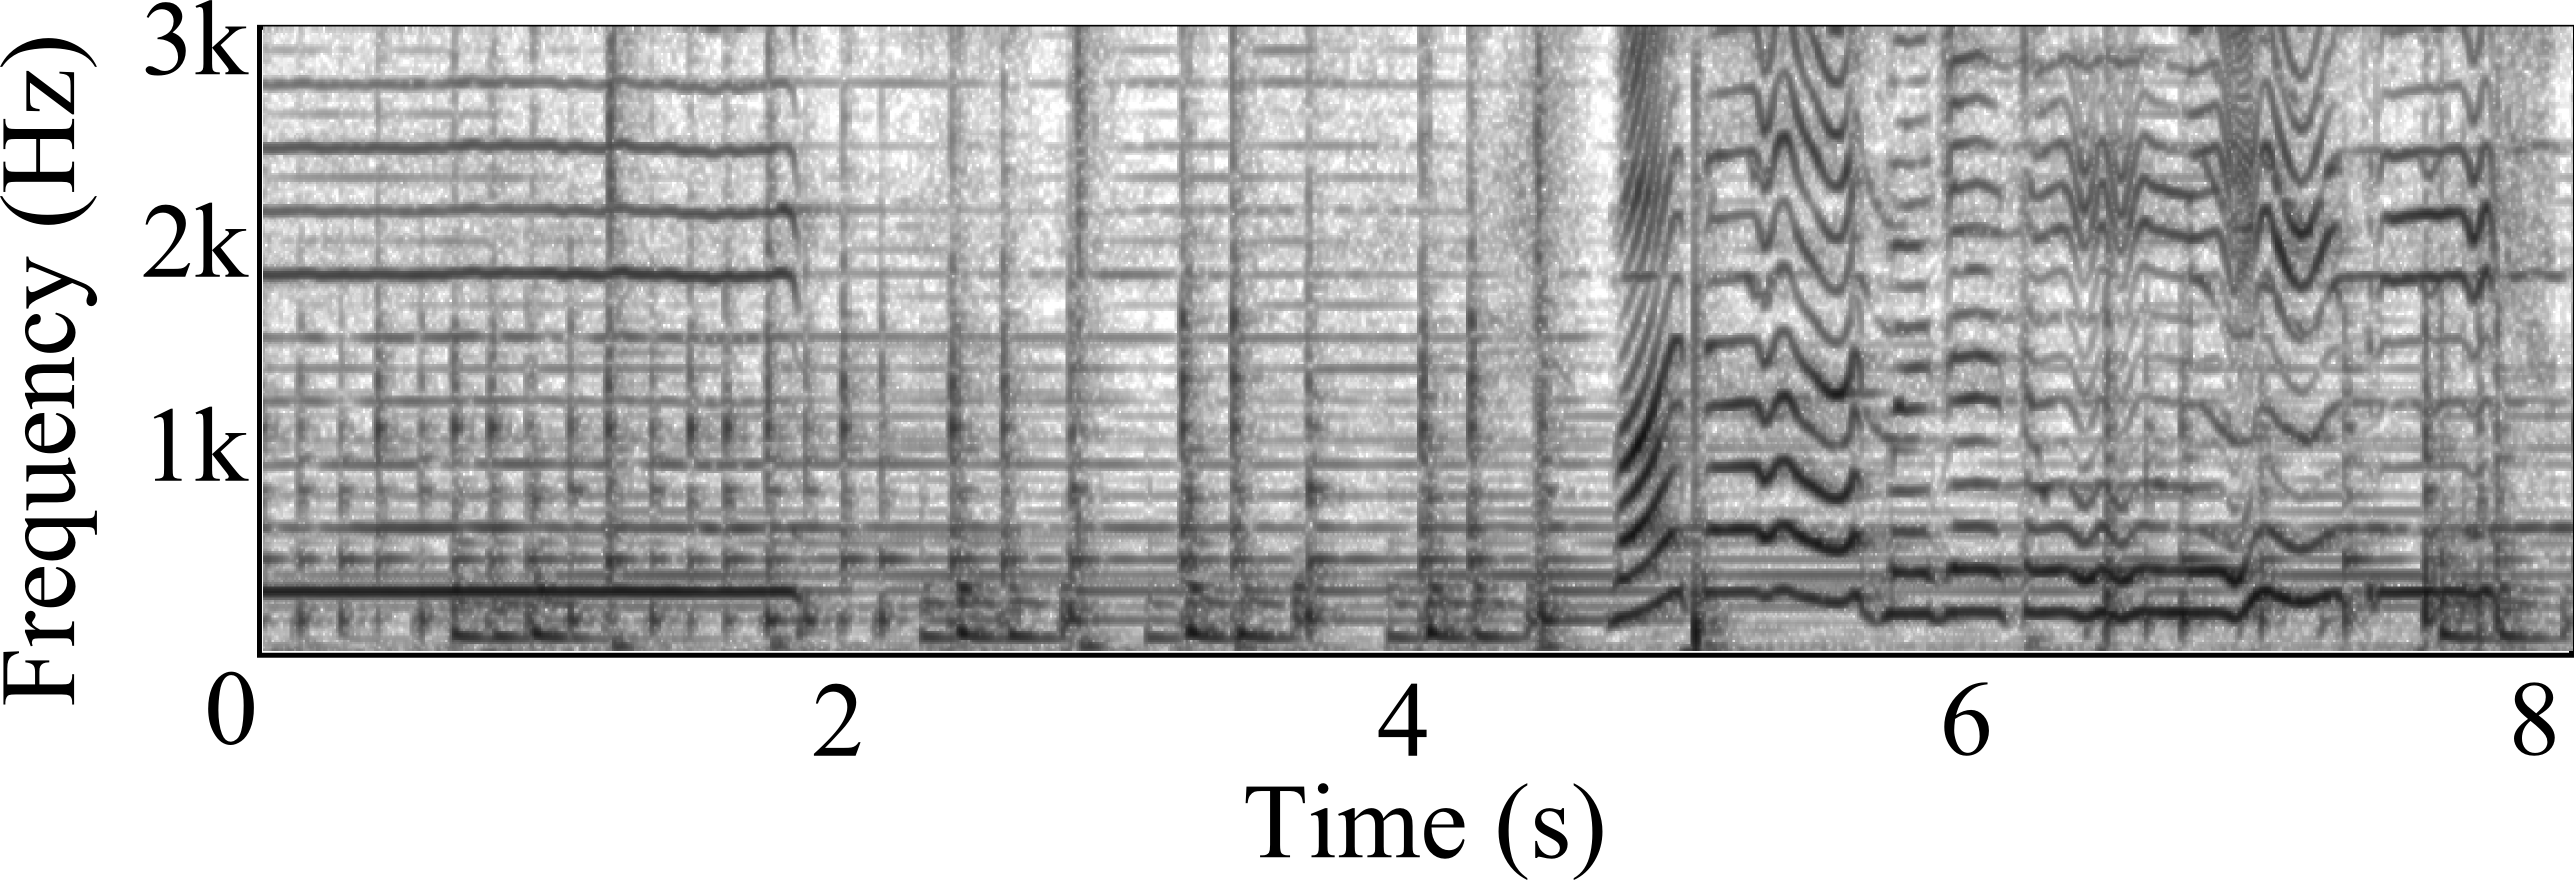
\includegraphics[width=0.99\textwidth]{percPatterns/carnatic-spectrum-proc.png}
    } \\ 
    \subfloat[Hindustani music]{\label{fig:sigdesc:hindustani}
      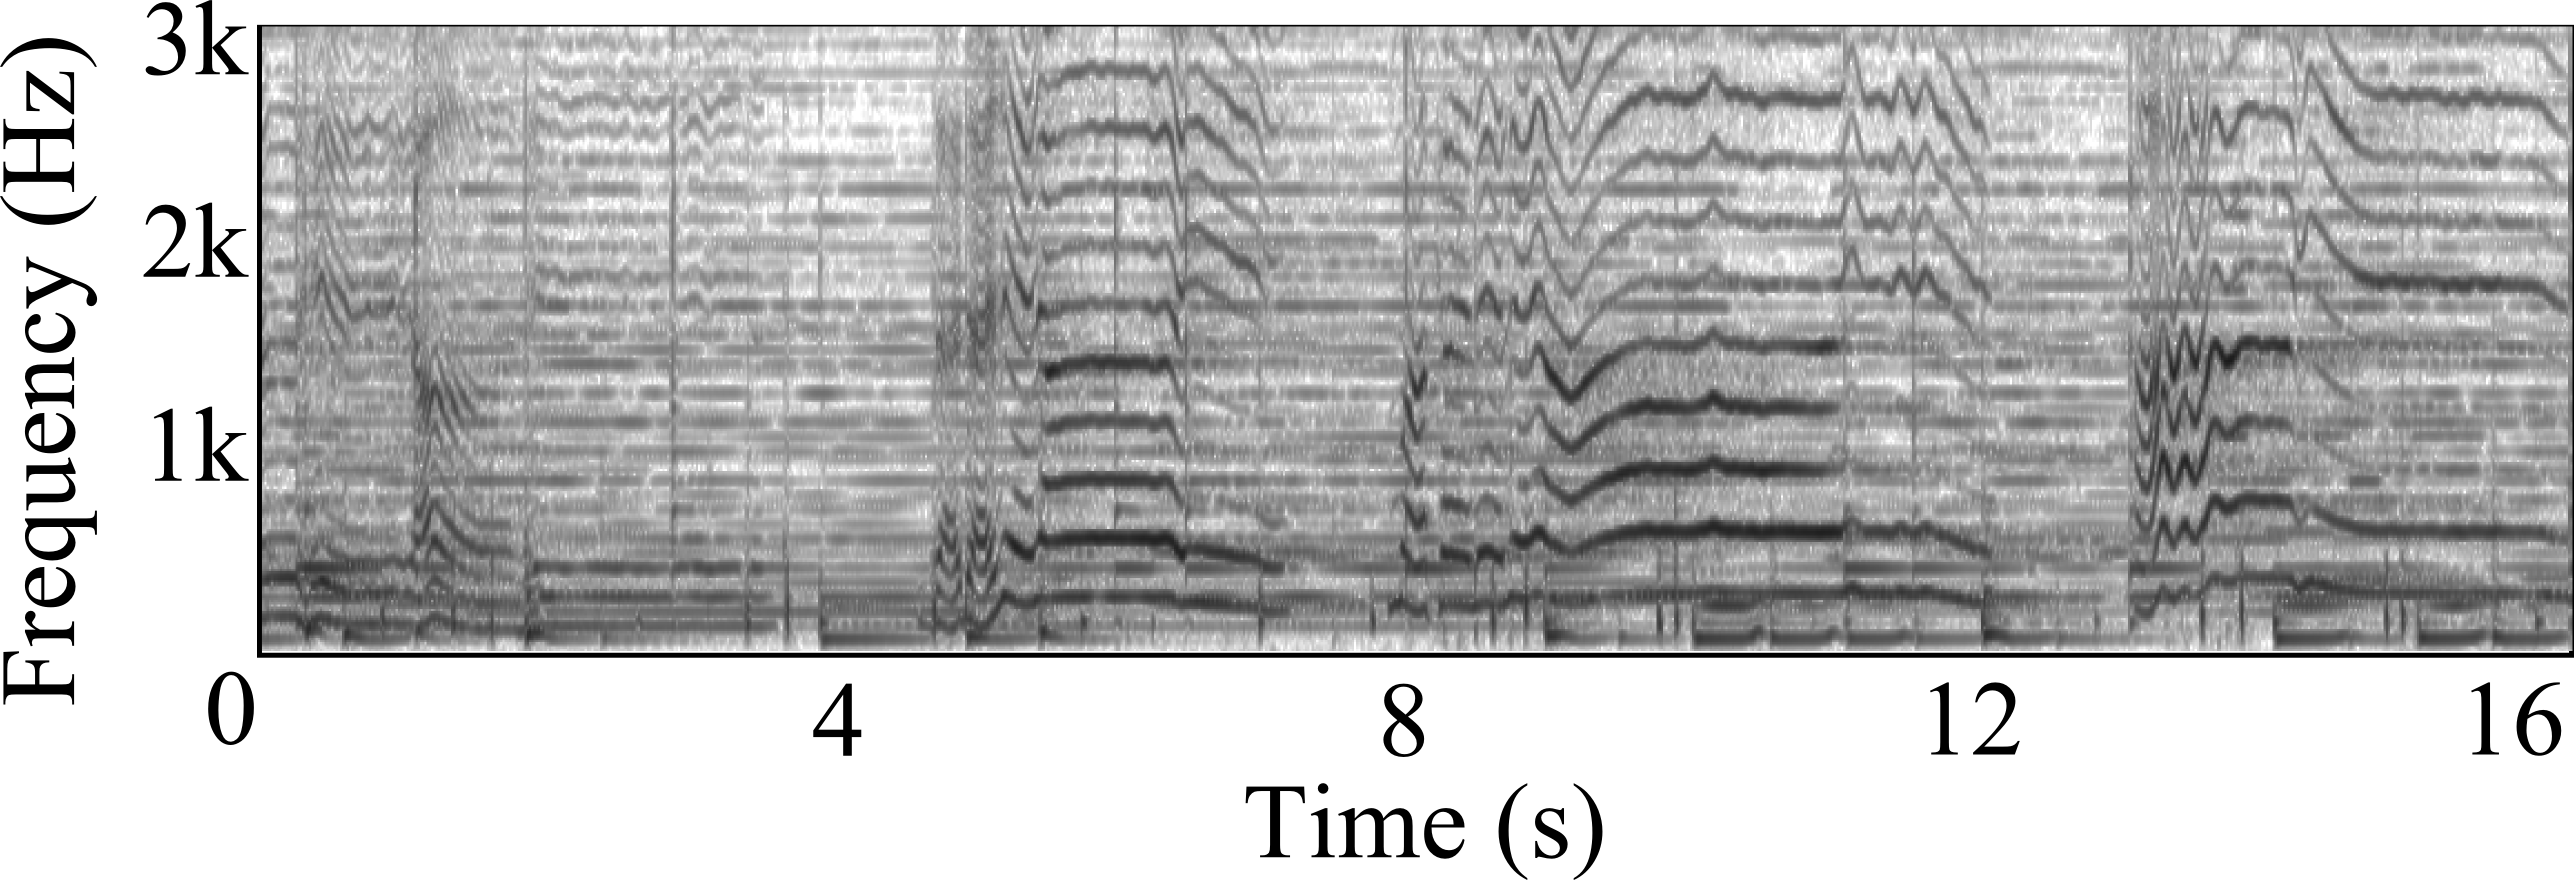
\includegraphics[width=0.99\textwidth]{percPatterns/hindustani-spectrum-proc.png}
    } 
\caption[Audio signal characteristics of Indian art music signals]{Audio signal characteristics of Indian art music signals. The figure shows the spectrogram of the audio excerpt of Carnatic and Hindustani music, showing the frequencies up to 3 kHz.}\label{fig:sigdesc:iam}
\end{figure}

The percussion instruments \gls{tabla} and mridangam have a bass drum head, and a treble drum head that is pitched. The pitched drum head is tuned to the tonic of lead musician. The pitched strokes can be sharp or sustained. Both the figures show the percussion strokes as vertical lines, showing their broad spectrum. We can identify the strokes from the left and right drums distinctly in different frequency ranges in both cases. In addition, we can see the some of the harmonics of the pitched percussion strokes, and the quick decay of the percussion strokes. The Hindustani excerpt is taken from a \gls{madhyam} \gls{lay} piece and we can see the longer notes and sparser \gls{tabla} strokes, indicating lower rhythmic density due to lower tempo. 
% \comment{Combining sources of information from melody and percussion can also aid automatic rhythm analysis. Using audio only, rhythm analysis can be supported by the phrasing of melodies, which is in most cases correlated with the \gls{tala} \update{citeXX}. For Indian music, tracking of the percussion strokes has a potential of increasing the accuracy of rhythm analysis.}
%
\section[Research problems in rhythm analysis]{Research problems in rhythm\\ analysis of Indian art music}\label{sec:probs:iamrhythm}
%\comment{For each problem, discuss its applications and list down a big ``picture" block diagram of what it encompasses.}For each problem discussed, discuss in brief the task, why its relevant, how it can be solved, are there any analogous approaches in Indian music, and then an evaluation if its present. \\ Problems to discuss: \comment{Check note book}
\begin{figure}
\centering
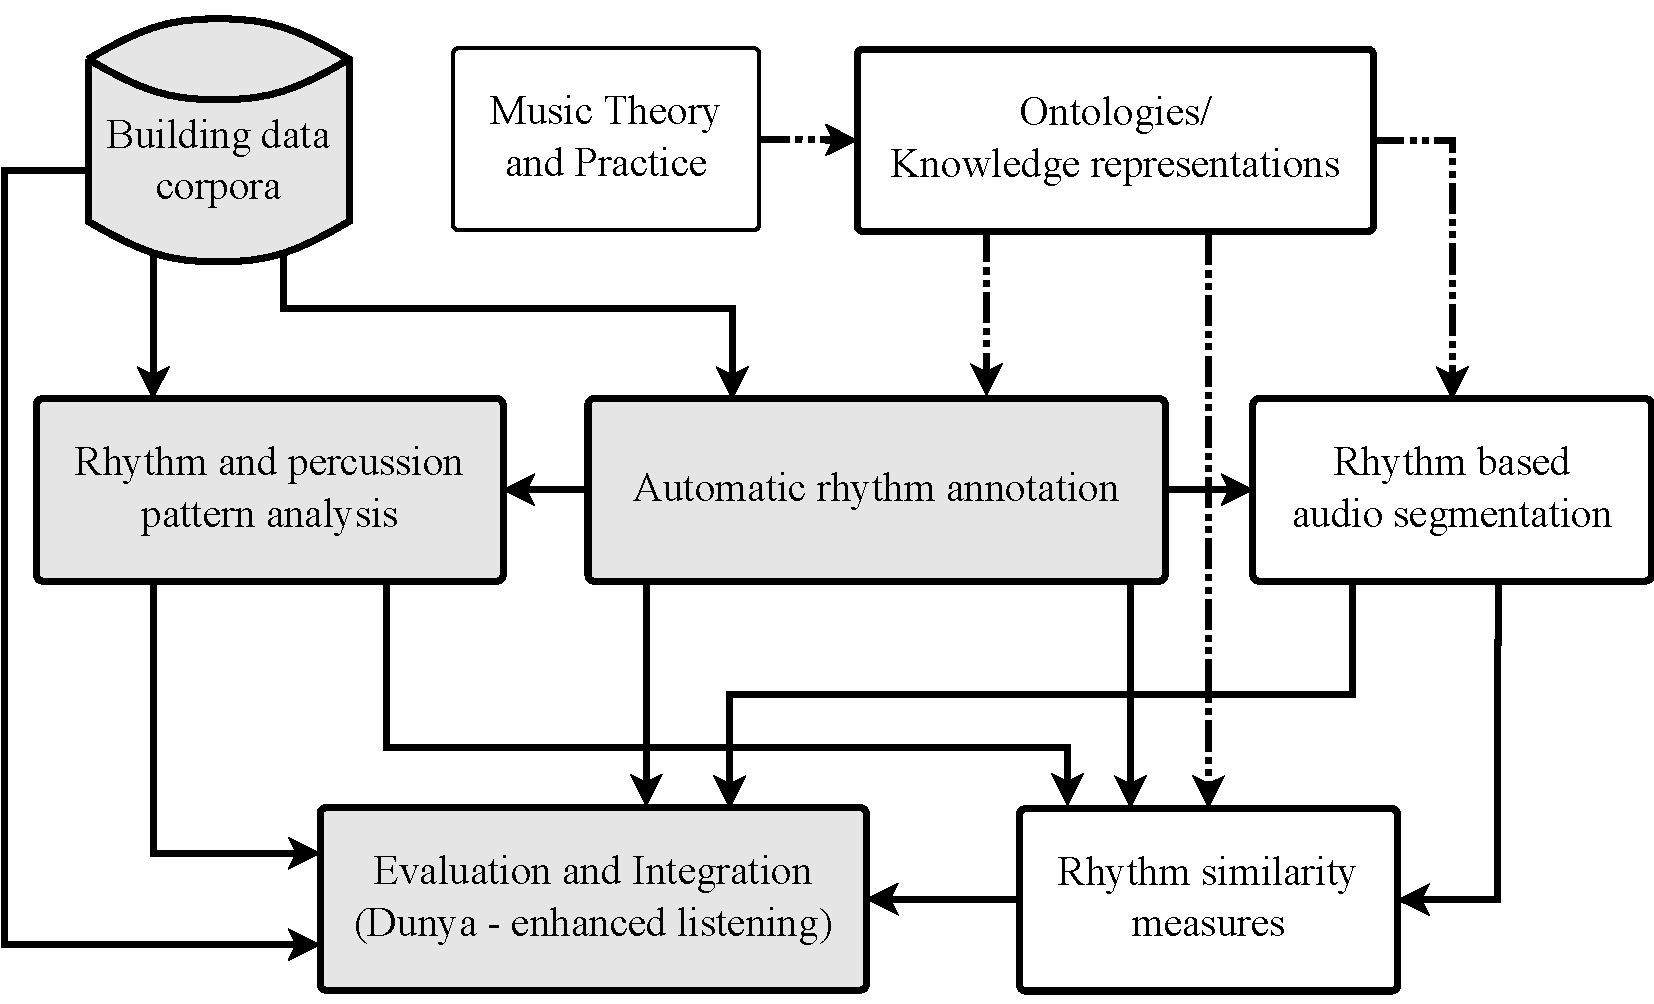
\includegraphics[width=\textwidth]{figs/blockDiags/ResearchProblems.pdf}
\caption[Relevant automatic rhythm analysis problems in Indian art music]{Relevant automatic rhythm analysis topics and applications in Indian art music. The solid lines indicate the flow of data and signals. The dot-dash lines indicate the flow of high level information such as parameters and priors. The subset of problems focused in this dissertation are shown in gray.}\label{fig:probdef:iamprob}
\end{figure}
With the background provided so far, several relevant and interesting automatic rhythm analysis problems in Indian art music are identified and discussed. For each problem, we briefly describe the problem, explain its relevance, identify any specific challenges, discuss possible approaches, and review any prior existing work for the problem. Some allied research problems not directly in the scope of rhythm analysis, but have related applications or could benefit from rhythm analysis are also discussed for the sake of completeness. Many of the rhythm analysis problems have not been addressed before, while there have been attempts in \gls{MIR} aiming to solve similar problems in Eurogenetic music. While some basic rhythmic feature extraction methods such as onset detection can be easily extended to Indian art music, more complex tasks have to reformulated with the context. Hence, some of the existing general rhythm descriptors such as onset detectors and tempo estimators are deemed to be useful to develop specific algorithms. % such as structural analysis and semnatic web technologies. 

Rhythm is characterized by structures and patterns. The structures provide the basis for patterns, through which rhythms are played. The problems presented here revolve mainly around these two concepts, and are categorized into several groups, with the final goal of using all these components to define musically meaningful and useful rhythm similarity measures for Indian art music. There are several sub-problems that lead towards the final goal. The problems span the whole range of complexity, starting from basic tasks processing the audio signal to abstract tasks requiring extensive music knowledge. The categorization of problems presented here is only for the purpose of presentation, and the problems in each category cannot be addressed in isolation. There is significant interplay and overlap between the groups - with problems benefiting from outputs of other problems in a different group, e.g. onset detection can help in both meter analysis and pattern discovery tasks. 

At the outset, from a literature review, we see that automatic rhythm analysis of Indian music has been attempted only recently, and concrete methods for Hindustani music and Carnatic music do not exist as yet. \citeA{Koduri:11:carnaticISMIR} also elucidate several unsolved problems in rhythm analysis of Carnatic music. \figref{fig:probdef:iamprob} shows an overview of the rhythm related research topics and applications Indian art music. It also shows the flow of data and information across the important units. The set of topics addressed in the dissertation are shown in gray. Each of those topics uses information and knowledge representations derived from music theory and practice, making them more informed and culture-aware. The data-driven approaches finally culminate with rhythm similarity measures computed from the data outputs from different automatic analyses. Each of the units are further described in detail, with sub-problems within them. 
%
\subsection{Building data corpora}
A significant part of data-driven research with signal processing and machine learning approaches needs good quality data. Data corpora that are representative of the music culture under study are essential for building and testing such approaches. The data sources comprise of audio, metadata accompanying audio, music scores, lyrics, manual and automatic annotations, and linked (semantic) data. One of the main problems addressed in this dissertation is building suitable data corpora for rhythm analysis research, a problem that is described further in \secref{sec:probdef:thesisdatasets}. Building useful datasets also involves building tools for rhythm annotation and developing machine readable representations for the annotations and metadata for effective linking and integration of these data sources. 
%
\subsection{Automatic rhythm annotation}\label{sec:probdef:autoannot}
%They annotate audio with: segments, events (such as beats, sama), annotation labels such as tala, lay, edupu, nade, time series (such a time varying pulse, et al.)
%Two levels: label generation for a piece: tala recognition, edupu, lay estimation, nade 
%Time aligned tracking: meter inference and tracking, 
Automatic rhythm annotation encompasses a broad set of problems that aim to annotate and tag audio recordings with several rhythm related metadata and tags. The tags could be descriptor tags that are not time aligned with audio, such as the tags related to the components of the \gls{tala} and median tempo descriptors. There could one or more such tags associated with each recording. The rhythm annotations could also be time aligned, indicating the locations of several rhythmic events in audio recordings, such as a time varying tempo, beats, and downbeats (\gls{sama}). The common tasks of tempo, beat and downbeat tracking can be classified as automatic rhythm annotation problems. 

Automatic rhythm annotation, in the context of Indian art music can be defined as the estimation of the characteristic components of the \gls{tala} from audio. For Carnatic music, the most important rhythm related tags include estimating the median tempo of the piece (in \glspl{akshara} per minute or beats per minute), the length of the cycle (in number of beats or \glspl{akshara}), the \gls{tala} label (and hence implicitly the underlying metrical structure), the \gls{nade} (and hence the subdivision structure), and the \gls{edupu} of the piece. For Hindustani music, the most important rhythm related tags include the median tempo of the piece (in \glspl{matra} per minute), the \gls{lay} class, the cycle length (in \glspl{matra}) and the \gls{taal} label. Estimating the time varying tempo curve, the \gls{akshara} pulse locations, the beats, the \gls{anga} (section) boundaries and the \gls{sama} instants are the important time aligned annotation problems in Carnatic music. The most important problems in Hindustani music are the estimation of the \gls{matra} pulsation, the \gls{vibhaag} boundaries, and the \gls{sam} instants. 

Automatic rhythm annotation is an important rhythm analysis topic, and there are several applications in which these rhythm annotations are useful, such as music autotagging, rhythm based segmentation of audio, beat aligned processing of music, audio summarization, music transcription, and different rhythmic pattern analyses. Tracking the components of the \gls{tala} through a music piece is essential for most other rhythm description tasks such as segmentation and extraction of rhythmic patterns to define similarity. Each of these problems are now described in detail. It is to be noted again that many rhythm annotation problems can be jointly addressed, estimating several components together, e.g. the \gls{tala}, tempo, beats and the \gls{sama} can be jointly estimated, in a task that we call as meter inference. 
% 
\subsubsection{\Gls{tala} recognition}
\Gls{tala} recognition\index{Tāḷa recognition}, defined as tagging an audio recording with a (possibly more than one) \gls{tala} tag is a central research problem of Indian art music. A \gls{tala} tag is the most basic information for listeners to follow the rhythmic structure of the music piece. As the most important rhythm related metadata associated with a recording, knowing the \gls{tala} is useful for archival, navigation, and enriched listening with large audio music collections of Indian art music. 

Since there are only a limited set of \glspl{tala} in Indian art music, \gls{tala} recognition can be formulated as a classification task based of features of the \gls{tala} estimated from audio. Barring a few exceptions, most compositions are composed in only one \gls{tala}, and hence an audio recording with the performance of the composition has only one \gls{tala} tag. However, audio recordings with long concerts with multiple compositions performed can have multiple \gls{tala} tags, with the additional problem of marking the regions of audio where these compositions are performed. Further, many recordings start with an \gls{alapana}, which is an unmetered section and hence has no \gls{tala}. Hence, \gls{tala} recognition has to first be preceded by such segmentation of audio recording into parts that have only one or no \gls{tala}. Exceptions can occur despite that, when some rare compositions can be performed in two different \glspl{tala}, a case that is uncommon and only has esoteric importance. Such marginal cases are beyond the scope of engineering approaches in this dissertation. 

\Gls{tala} recognition is a subjective task that needs prior music knowledge. It can be achieved through a set of proxy tasks, all of which help in identifying the \gls{tala}. The clues to identifying a \gls{tala} are related to its structure and the rhythmic patterns played in it. The patterns (such as the \gls{theka}) played are indicative of the \gls{tala}, but many patterns are also shared across many \glspl{tala}. From an \gls{MIR} perspective, it is harder to recognize these patterns, but instead, it is easier to recognize these patterns if the \gls{tala} is known, creating a circular dependency. 

The structure attributes of the \gls{tala} that can be used to identify the \gls{tala} are the cycle length and when defined, the subdivision meter (in Carnatic music). Estimating the cycle length in beats (or \glspl{matra}) can help significantly to identify the \gls{tala}. However, there are several \glspl{tala} in both Carnatic and Hindustani music that have the same length, e.g. \gls{ektal} and cautāl both have 12 \glspl{matra} in a cycle~\cite{clayton:00:time}, and hence additional information is needed to disambiguate them. Nevertheless, cycle length estimation is an important task that has received some attention from the research community, with the analogous tasks in Eurogenetic music being time signature estimation and meter estimation. 

In Indian music, we can track well-defined cycles at several levels of the meter. As described earlier, though the aim of the task is to estimate the length of \gls{tala} cycle (length of a \gls{avart}/\gls{avartana}), the algorithms might track a different time scale, which need not correspond to the \gls{tala} cycle. One such other specific level of interest apart from the \gls{tala} cycle is the division within the beat pulsation, i.e. the periodic structure dominating the rhythmic content between the beat instances. In Carnatic music, this corresponds to the \gls{nade} estimation. Further, we need to point out here that there is a clear definition of the subdivision meter in the form of \gls{nade} in Carnatic music. However, such an explicit subdivision meter for Hindustani music is not clearly given by the theoretical framework. 

Though the \gls{tala} cycle is an important part of rhythmic organization, it is not necessary that all phrase changes occur on the \gls{sama}. In \gls{adi} \gls{tala} for example, most of the phrase changes occur at the end of the 8 beat cycle, there are compositions where some phrase changes and strong accents occur at the end of half-cycle or the phrase might span over two cycles (16 beats). 

Since the \gls{tala} cycles have a periodicity, prior approaches in Indian art music track the periodicity in pulsation. \citeA{sankalp:11:meter_short} and \citeA{sankalp:12:meter} proposed a method for meter detection from audio for Indian music, and classify a piece as belonging to duple (2/4/8), triple (3/6), or septuple (7) meter. A mel-scale frequency decomposition of the signal is used to drive a two stage comb filter bank. The filter bank output is used to estimate the subdivision time-spans and the meter of the song. It was tested on an Indian film music dataset with encouraging results. This is one of the first proposed approaches to rhythm modeling applied specifically to Indian music. However, the algorithm was tested on a different repertoire than Hindustani and Carnatic music. The algorithm only aims to classify into these broad meter classes and does not attempt to assign a \gls{tala} label, which is more complex than such a classification. Though proposed for Indian music, the algorithm is general in approach and does not consider any specific characteristics of rhythm in Indian music. \citeA{miron:11:thesis} addressed the problem of \gls{taal} recognition in Hindustani music, based on recognizing the \gls{theka} played on the \gls{tabla}. Using a labeled corpus of Hindustani music with \gls{tabla} accompaniment, he explored segmentation and stroke recognition in a polyphonic context, and concluded that recognizing Hindustani \glspl{taal} is a challenging task. 

\citeA{ajay:12:beatWkShop} also proposed a culture-specific beat tracking based approach to \gls{tala} description, and applied it to Carnatic music. They proposed a system to describe meter in terms of the time-span relations between pulsations at bar, beat and \gls{akshara} levels. The tempo estimation in the algorithm, which is adapted from the algorithm by \citeA{davies:07:beat}, is modified to peak at 90 \bpm\, allowing a wide range of tempi (from 20 bpm to 180 bpm) to be estimated. The algorithm applies the beat tracker proposed by \citeA{ellis:07:beat} with the estimated tempo as input. The algorithm then uses a beat similarity matrix\index{Similarity matrix} and \gls{IOI} histogram to automatically extract the sub-beat structure and the long-term periodicity of a musical piece, from which a set of rank ordered candidates could be obtained for the \gls{nade} and \gls{avartana} length. The algorithm was tested on a manually annotated Carnatic music dataset consisting of 86 thirty second song snippets of both vocal and instrumental music with different instrumentation, set to different \glspl{tala} and \gls{nade}. The algorithm was also tested on an Indian light classical music dataset consisting of 58 semi-classical songs based on popular Hindustani \glspl{raga}. Though formulated using the knowledge of the \gls{tala}, the algorithm does not make an effort to resolve metrical level ambiguities, which can severely affect the accuracy since the performance of the algorithm depends mainly on reliable beat tracking at the correct metrical level.

Rhythmic similarity can also be used in \gls{tala} recognition, with the assumption that the rhythmic patterns played in a \gls{tala} across recordings are similar. Rhythmic similarity can be applied to the task by assigning an unknown piece to a class of rhythm it is deemed to be most similar to, based on some low level signal features. Given \gls{tala} annotated audio examples, rhythmic features can be extracted from audio and used to learn models of rhythm similarity that can classify \glspl{tala}. If the classes of rhythm present in a collection have distinct cycle lengths, we can also obtain the length of the cycle for an unknown piece through this classification. 

Practically, most commercially released music collections provide the \gls{tala} of each piece as editorial metadata. The name of the \gls{tala} is present in most pieces in the collection. However, it is often not present in archived recordings, personal music collections, or open music collections. Since most of the work in this dissertation is with commercial music recordings, we already have access to \gls{tala} tags of these music recordings and hence the task of \gls{tala} recognition is redundant and not relevant with these collections. Further, manually curating audio collections with \gls{tala} tags is less time consuming and less resource intensive than tasks such as tempo and beat tracking. Hence, we do not work explicitly on \gls{tala} recognition problem in this dissertation, but however, it is expected to be a byproduct of other automatic rhythm annotation tasks.
%
\subsubsection{\Gls{lay} classificaion in Hindustani music}
With the wide range of tempo divided into tempo classes, \gls{lay} classification into \gls{vilambit}, \gls{madhyam} and \gls{dhrut} (and possibly more extended ranges of \gls{lay} classes) is a useful problem. Since surface rhythm is not an accurate indicator of the underlying tempo, a knowledge of the \gls{lay} class can significantly help in reducing metrical level errors in tracking the tempo and the \gls{taal}. Since surface rhythm can be misleading, \gls{lay} classification needs to combine features from melody and identify specific \gls{tabla} stroke timbres to determine the actual underlying tempo class. 
% 
\subsubsection{\Gls{edupu} estimation in Carnatic music}
\Gls{edupu} estimation in Carnatic music is a unique problem. Though the \gls{edupu} is a metadata of the composition, unlike the \gls{tala} label, it is never recorded as standard metadata and hence needs estimation. When not available as metadata, \gls{edupu} estimation needs to be addressed based on accents and salience of the beats and their correlation with the lyrics and melodic phrases. Estimating \gls{edupu} might be necessary for correct alignment of the \glspl{sama} since in pieces with a non-zero \gls{edupu}, it is likely that the melodic changes tend to occur at the \gls{edupu} point rather than at the sama of the \gls{tala} cycle. This might lead to confusion in sama tracking algorithms. We also noticed that non-zero \gls{edupu} pieces tend to give poorer performance in tasks such as cycle length recognition \cite{ajay:14:rhythmJNMR}. However, with a robust \gls{sama} tracking algorithm which can handle different rhythmic patterns, the effect of non-zero \gls{edupu} is less. To the best of our knowledge, this problem has not been addressed by the research community so far. Since the problem of \gls{edupu} estimation is very specific to Carnatic music, it is of limited interest and is not addressed in this dissertation. But when required, we will examine the effect of non-zero \gls{edupu} on other rhythm analysis tasks. 
%
\subsubsection{\Gls{tala} tracking}
\Gls{tala} tracking (or generally meter tracking)\index{Meter analysis} refers to a set of problems that aim to estimate the different components of the \gls{tala} (the metrical structure) over time in an audio recording, and estimate several time aligned annotations related to the meter. By tracking these \gls{tala} components, a complete description of the metrical structure of the piece at different hierarchical levels can be achieved - tracking the cycles as described by the theoretical framework over time. From such a task, all the components such as tempo, \glspl{akshara}, beats and \glspl{matra}, sections, and \gls{sama} can be obtained. \Gls{tala} tracking is an important automatic rhythm annotation task and is the first step towards any further structural analysis of music pieces. 

\Gls{tala} tracking can be done without any prior knowledge of the music piece, in which case identifying the \gls{tala} is an implicit step in the process. We call such an uninformed tracking as meter inference\index{Meter inference} - to identify the meter type, and estimate the time varying tempo, beats and the \gls{sama} (downbeats) all together. The \gls{tala} tracking algorithms can greatly benefit from knowing the \gls{tala}, tracking a known metrical structure. We call such a task as meter tracking\index{Meter tracking} (in contrast to meter inference) - given the \gls{tala}, estimating the time varying tempo, beats, and downbeats. We can categorize the sub-tasks in \gls{tala} tracking as tempo tracking, beat tracking, and \gls{sama} tracking. 

\textbf{Tempo tracking}: Tempo tracking\index{Tempo tracking} aims to estimate the time-varying tempo over the audio recording of a music piece, measured in \glspl{akshara}/beats/\glspl{matra} per minute. The knowledge of time-varying tempo is useful to track the beats. Even a good estimate of median tempo helps in tracking the beats at the correct metrical level. Median tempo is a good indicator of tempo and can be used as a rhythm tag on a music piece. As described earlier, the tempo changes both locally and over longer periods of time, and the algorithms for tempo estimation need to be robust to these changes. 

\textbf{Beat tracking}: In the context of \gls{MIR}, as noted earlier, beat tracking\index{Beat tracking} is commonly defined as determining the time instances where a human listeners are likely to tap their foot to the music. This definition is likely to cause problems in our context, as for example in Carnatic \gls{khanda chapu} \gls{tala}, listeners familiar to the music tend to tap an irregular sequence of pulses, at the section level, instead of the faster regular pulsation. Also, depending on the \gls{lay}, listeners of Hindustani music tap on either the \gls{matra} level for \gls{vilambit} and \gls{madhyam} \gls{lay}, or at the \gls{vibhaag} level for \gls{dhrut} \gls{lay} \cite[p.~91]{clayton:00:time}. In such a case, the more appropriate task of tracking the possibly irregularly spaced beats is more relevant for Indian art music.

Despite these ambiguities, we pursue the task in the present context using a more adapted definition of a beat for the purpose of consistency, defined as a uniform pulsation defined at the ``beat" (as defined in \secref{sec:bkgnd:carRhythmIntro}) level for Carnatic music, and at the \gls{matra} level for Hindustani music. This definition of an equidistant beat pulsation can later help in deriving the musically relevant possibly non-isochronous beat sequence that is a subset of the equidistant pulses. The possibly irregular pulse sequence is a subset of the uniform pulsation estimated from the algorithms. This approximation is further inconsequential if the whole cycle along with the \gls{sama} are tracked, using which any pulsation within the beat - uniform or non-uniform can be derived out of that information. The \gls{vibhaag} or \gls{anga} boundaries also coincide with a subset of the beats and hence can be derived from the estimated beat locations. A task that is specific to Carnatic music is \gls{akshara} pulse tracking, estimating the subdivisions of the beat, an algorithm for which is elaborated in \secref{sec:mt:earlyexpts}. 

\textbf{Sama (downbeat) tracking}: The information about where a \gls{tala} cycle begins provides us with the ability to comprehend most of melodic, rhythmic and structural development of a piece, which is typically synchronized with the phase of the \gls{tala} cycle. This corresponds to detecting the \gls{sama} (or \gls{sam}) instants of the \gls{tala} cycle. In Hindustani music, the \gls{sam} is highly significant structurally, as it frequently marks the coming together of the rhythmic streams of soloist and accompanist, and the resolution point for rhythmic tension \cite[p. 81]{clayton:00:time}. In Carnatic music, most of the phrasing and improvisations, both melodic and rhythmic, are tied with the \gls{sama} and hence its relevant and meaningful to explore tracking the \gls{sama} as a primary problem in automatic rhythm annotation. 

Note that while the term downbeat has been mostly applied to eurogenetic music, we apply it here as well because it generally denotes the pulse at the beginning of a bar. The downbeat does not necessarily correspond to the strongest accent in the cycle. In this sense, downbeat in Indian art music and Eurogenetic music are likely to be concepts with different meaning. 

It is to be noted that all the above components can be tracked together jointly, instead of individually. Such meter tracking algorithms are an important focus of the dissertation. Automatic rhythm annotation one the main topics of this dissertation, and a subset of the problems described above form the subject matter of \chapref{chap:meterInfTrack}. To the best of our knowledge, the problem of meter tracking for Indian art music is addressed for the first time in this thesis. The subset of problems that will be explored deeper in this dissertation are better formulated in \secref{sec:probdef:thesismeter}.
%
\subsection{Rhythm and percussion pattern analysis}
While \gls{tala} provides a framework and structure, the rhythm and percussion patterns form the content through which the metrical structures and rhythms are illustrated, and hence form the other main component of rhythm analysis. Rhythm patterns mainly refer to the temporal arrangement of different events with different accents, while percussion patterns include a temporal arrangement of different percussion timbres. To contrast, percussion patterns are rhythmic patterns, but rhythmic patterns need not contain only percussion, and can be formed by melodic and/or percussion instruments. 

A pattern is defined as a temporal sequence of events and hence it is necessary to estimate onsets of various instruments in music, since that creates the time-aligned sequence of note/stroke events that can be further used to obtain both rhythmic and percussion patterns. Some important sub-problems within pattern analysis are instrument-wise onset detection, pattern transcription, and pattern discovery, each of which is described further. Transcription aims to map an audio recording into a time aligned sequence of symbols (strokes, accents, e.g.). The problem of discovery is more open ended and aims to automatically retrieve interesting patterns and insights about those patterns, in a data-driven way. 
%
\subsubsection{Instrument-wise onset detection}
The task of instrument-wise onset detection\index{Onset detection} refers to detecting the onsets of specific instruments from an audio signal that is a mixture of many music instruments and was described in \secref{sec:bkgnd:onsetdetect}. For rhythm analysis in Indian art music, instrument-wise onset detection can help to obtain cues for both meter tracking and for analysis of percussion patterns. The onsets of percussion instruments mridangam and \gls{tabla} provide cues to the \gls{tala} and delimit percussion patterns. A differentiation between the left (bass) and right drum onsets in both instruments is additionally insightful and useful. Instrument-specific onsets are often not estimated explicitly, but are estimated as a part of a bigger task, such as percussion transcription. % An allied problem of the task is instrument tracking, which aims to provide a time varying activation curve that indicates the time stamps where each of the instruments are active and can help in structural segmentation. 

It is a difficult task to extract out percussion onsets with a great accuracy, given that the percussion in Indian art music is also tuned and shares the same frequency range as the melody. Within CompMusic, instrument-wise onset detection has been explored for Beijing opera~\cite{tian:14:icassp}. \Gls{HPSS} can help to improve onset detection of percussion instruments (\secref{sec:bkgnd:onsetdetect}) and has been applied to Carnatic music by \citeA{ajay:14:talaTrack} with limited success. Given the complexity of the task, it is preferable to build models that are robust to errors in onset detection of specific instruments. 
%
\subsubsection{Rhythm pattern analysis}
Rhythm patterns extracted from audio recordings are representative patterns of the \gls{tala}, and hence useful for both automatic \gls{tala} recognition and meter tracking. The most relevant rhythmic patterns are cycle length rhythmic patterns - patterns that are played in one full cycle of the \gls{tala}. Shorter patterns, played within a cycle mostly act as rhythmic atoms to make up the whole cycle and are played more often. However, there are long rhythmic patterns played on mridangam/\gls{tabla} and accentuated through melody that can last many cycles. Automatic discovery of rhythm patterns can be used to define content based rhythmic similarity between pieces of music, which is expected to be more relevant than metadata based similarity. Automatic extraction of rhythm patterns can also be a tool for musicologists to study various rhythm patterns in larger corpora. 

Rhythmic patterns are closely tied to the \gls{tala}, and within a \gls{tala} cycle to the sections of the cycle. Hence, a pattern discovery system can significantly benefit from all forms of \gls{tala} related metadata. Consequently, rhythm pattern discovery needs \gls{tala} annotated (with time-aligned \gls{sama} and beats) datasets for a better performance. A systematic study of rhythm patterns in Indian art music is lacking, and an illustrative effort towards that is a part of the dissertation (\secrefs{sec:cmrdataset}{sec:hmrdataset}). 
%
\subsubsection{Percussion pattern transcription and discovery}
Percussion pattern \index{Percussion pattern}transcription is mainly applied on audio recordings with percussion solo, and aims to transcribe the audio recording into a time-aligned sequence of drum stroke labels, and in the case of Indian art music, into percussion syllables. Percussion transcription is a sub-problem of the more general music transcription. Transcription of a solo into symbolic syllables is an example of audio segmentation at a fine grain level. Transcription of solo performances are useful for percussion training. Since Indian art music is mostly improvised, the need for such a fine grained transcription system is limited, except for music education and performance analysis applications. However, a transcription can be used to automatically discover percussion patterns and develop rhythm similarity measures using such discovered patterns. 

The use of oral mnemonics is not unique to Indian art music. Many music traditions around the world have developed particular systems of oral mnemonics for transmission of the repertoire and the technique. \citeA{hughes:00:syllable} coined the term \textit{acoustic-iconic mnemonic} systems for these phenomena\index{Oral mnemonic syllable}, and described their use in different genres of traditional Japanese music. As he points out, the core aspect of these systems is that the syllables are chosen for the similarity of their phonetic features with the acoustic properties of the sounds they are representing, establishing an iconic relationship with them. Therefore, these systems are essentially different from those of solmization\index{Solmization} \cite[accessed June 2016]{hughes:14:grovesolmization}, like for instance the syllables of solfège, of the Indian svaras (notes) or the Chinese gongche notation, which are nonsensical in relation to the acoustic phenomena they represent. 

The use of the aforementioned systems for the transmission of percussion is wide extended among many traditional musics. \citeA{hughes:00:syllable} mentions the \textit{shōga} used for the set of drums of \textit{Noh} theatre. In Korea, the young genre of \textit{samul nori}, a percussion quartet of drums and gongs, draws on traditional syllabic mnemonics for the transmission of the repertoire. Furthermore, these systems are also known to be used in Turkish traditional music and Javanese music. 

The benefits of using oral syllabic systems from an \gls{MIR} perspective are both the cultural specificity of the approach and the accuracy of the representation of timbre, articulation and dynamics. The characterization of these percussion traditions need to consider elements that are essential to them such as the richness of their palettes of timbres, subtleties of articulation, and the different degrees and transitions of dynamics, all of which is accurately transmitted by the oral syllables. 

As discussed earlier, the onomatopoeic percussion system in Indian art music provides a language for percussion and hence is the most musically meaningful way to represent percussion patterns of \gls{tabla} and mridangam. Such a link between drum patterns and natural language has been explored by \citeA{mauch:12:patterns}. However, there are some challenges to percussion transcription in Indian art music. The syllables of \gls{tabla} and mridangam are not unique across all the schools. Since these syllables closely mimic the timbre and dynamics of the drum stroke, the mapping between the strokes to syllables is not unique and one to one, with several different syllables mapping to one stroke timbre. Further, within a percussion solo, a syllabic pattern can also be loosely interpreted, leading to further complexity. 

Percussion pattern transcription can be formulated as a supervised learning task, using labeled training data to build syllable stroke models, which can then be used to transcribe a test recording. Percussion pattern discovery is an unsupervised task, aiming to extract percussion patterns from audio and/or scores in an unsupervised way, though some priors can be used. Music scores of percussion solos (represented by syllables) are used for percussion training. Such scores can be used for symbolic analysis of percussion patterns, and used to discover percussion patterns from score corpora, a task that much less complex than extracting them from audio. We can then use these patterns and search for them in longer percussion solo recordings. Such an approach with pattern discovery from scores followed by pattern search in audio is explored further in this dissertation. 

A scientific study of Indian percussion instruments can be traced back to the study of acoustics of Indian drums by Sir C. V. Raman \cite{raman:20:drum, raman:34:drums}. In the last decade, most of the \gls{MIR} work with Hindustani music percussion has focused on drum stroke transcription, creative modeling for automatic improvisation of \gls{tabla} and predictive modeling of \gls{tabla} sequences. The first attempt at \gls{tabla} stroke transcription was done by \citeA{gillet:03:tabla}, with their more recent work mainly on sequence modeling of rhythm sequences~\cite{gillet:07:seq}. Parag Chordia \cite{chordia:05:phdthesis,chordia:05:tablaSeg} focused on automatic transcription of strokes from solo \gls{tabla} music. He developed a new encoding scheme for transcription of \gls{tabla} bols called the \texttt{**bol} format based on the humdrum syntax~\cite{huron:02:humdrum}. \citeA{rae:10:tablagyan} developed an automatic \gls{tabla} improviser. Extending further, most of work using \gls{tabla} sequences has been in a predictive modeling setup using the multiple viewpoint modeling framework \cite{chordia:10:mvmacm,chordia:11:predTabla,chordia:10:mvmismir,sastry:11:thesis}. \citeA{miron:11:thesis} explored segmentation and transcription of \gls{tabla} strokes within the context of \gls{taal} recognition in Hindustani music. 

The work with Carnatic percussion has been limited so far. Motivated by the work of \citeA{raman:34:drums}, \citeA{akshay:13:mridangam} used a \gls{NMF} based approach to decomposition of mridangam strokes into its modes, and used them for transcription. The work was further extended using cent-filterbank based features to make the transcription approach independent of the tonic \cite{akshay:14:transcription}. More recently, \citeA{kuriakose:15:mridangam} proposed an algorithm for mridangam stroke transcription and evaluated it on an annotated dataset of mridangam solos (see \secref{sec:mridangamdatasets} for the dataset). Percussion pattern transcription and discovery in both mridangam and \gls{tabla} solos is one of the problems addressed in the dissertation and is formulated more comprehensively in \secref{sec:probdef:thesispattern}. 
% 
\subsection{Rhythm based audio segmentation}
Segmentation\index{Segmentation} problems refer to a broad category of problems which involve the labeling segments of audio with a label/tag. Segmentation can be done at several levels, based on different music concepts. Segmentation problems are useful since they provide additional metadata to navigate through music collections (and within a single recording), and to further develop similarity measures. Audio segmentation is not the main focus of the dissertation, but several rhythm related segmentation problems are briefly described for completeness. 

A music recording can be segmented based on the instruments that are playing, a problem that can also be described as instrument tracking in audio. In Indian art music, this is useful to segment a piece into structural segments that are known to have specific instruments, e.g. an \gls{alapana} only has melodic instruments playing, while a percussion solo only has percussion instruments. In the context of Indian art music, \citeA{ranjani:15:instID} recently proposed an approach to track different instruments from a mixture. 

Segmentation can also be refer to segmenting a concert into the pieces that were performed in it, which is useful for archival. Segmentation at a structural level within a piece aims to segment the piece into different sections of the piece, and is useful for navigation and similarity. An applause based segmentation of Carnatic music concerts was proposed by \citeA{sarala:13:concertseg}, which was also extended to intra-piece segmentation into sections of a piece. Hindustani \gls{khayal} music concert recordings are often presented as a single recording with multiple pieces, performed in possibly different \gls{lay} and \gls{taal}. Segmenting Hindustani concert recordings based mainly on rhythm features using a modified tempogram was proposed by \citeA{vinutha:14:frsm}, and structural segmentation using additional audio features was proposed by \citeA{verma:15:concertseg}. A recent approach to estimate reliable tempo that aids in rhythmic segmentation was applied to \gls{sarod} concerts by \citeA{vinutha:16:sarod}. A rhythm based segmentation of such an audio recording is also useful for \gls{tala} tracking on the recording. Tempo or \gls{lay} class based segmentation can use a novelty function for onset detection and detect changes in tempo to segment audio.

Segmentation of recordings at the time scale where we can define meaningful rhythmic phrases is relevant. The span of these phrases are closely tied to the metrical positions of the \gls{tala} cycle. These phrases can characterize the rhythm of the piece and would be instrumental to measure rhythmic similarity between two pieces of music. Given some form of automatic rhythm annotations, such as the sama and the beats, extracting rhythmic patterns and rhythm phrase boundaries in the music piece, e.g. \gls{theka} segmentation aims to segment the piece at \gls{theka} changes. More generally, it encompasses the task of segmentation at rhythm phrase changes. Further, though the \gls{tala} of a song is fixed, the \gls{nade} could change through the song, and \gls{nade} based segmentation of audio would be further useful for structure segmentation of the song. Rhythm in both Carnatic and Hindustani music is highly improvised with a possibility of wide variety of rhythms. However, there are regions in the music piece with well defined structures that contain rhythmic phrases characteristic of the \gls{tala}. Identifying these ``regions of stable rhythm" would be helpful in rhythm annotation tasks. Further, these stable regions can be used to extract representative rhythm templates for measuring rhythmic similarity. 
%
\subsection{Ontologies for rhythm concepts}
Though not a topic addressed in the dissertation, ontology engineering (also called as knowledge engineering) aims to integrate human knowledge into computer systems to solve complex problems that require human expertise \cite{brachman:04:ontology,gomezperez:04:ontology,berners:01:semantic}. An ontology\index{Ontology} specifies concepts, attributes, relations, constraints, and instances in a domain. Since music is a complex and varied phenomenon with many perspectives, a cultural domain specific ontology is needed to define the relationships that pertain to a specific type of music. 

\Gls{tala} ontologies are knowledge representations of rhythm. They encode the relationships that exist among the rhythm concepts in Indian art music. Built using the knowledge of music theory and practice, the ontologies would be useful for querying complex rhythmic relationships between the pieces. The ontologies complement the features derived from the data with music knowledge based relationships that can be used for defining rhythmic similarity, e.g. using a \gls{tala} ontology and the knowledge of cycle length, it might be easier to identify the \gls{tala} from audio. Further, the ontologies will also be useful to create specific models with priors obtained from the ontology. In summary, ontologies can be built both for a direct use in navigation and inference, and for building domain specific machine learning algorithms. 

Previous work on ontologies have been mainly on organizing music and metadata \cite{swartz:02:musicbrainz,raimond:08:phd}. The CompMusic project aims to develop ontologies for all the music cultures under study, some examples include the work by \citeA{koduri:13:ontoMelody} and \citeA{koduri:14:ontoIntonation}. Building comprehensive ontologies needs expertise in music theory and ontology languages, an effort that is beyond the scope of this dissertation. In this dissertation however, we use basic knowledge representations to incorporate prior information in several rhythm analysis tasks. 
% 
\subsection{Rhythm similarity measures}
Rhythm similarity\index{Rhythm similarity} measures aim to use rhythm descriptors, metadata and segmentation information to provide an objective similarity value between two phrases, two music pieces, or two parts of the same piece. Developing culture-aware similarity measures is one of the final goals of the CompMusic project, and rhythm similarity is a major component of it. Since rhythmic similarity is not a very concrete notion, we need definitive and objective measures of similarity, especially in a multicultural setting. This would necessitate the use of knowledge based approaches for similarity modeling. An in-depth study of rhythm similarity measures is not a part of the dissertation. However, some possible directions of research towards the goal are discussed. 

The onus of developing new similarity measures clearly lie on the choice of metrics that correspond to rhythm similarity as perceived through musically relevant concepts - based on \gls{tala} and the rhythmic patterns. The \gls{tala} ontologies provide the empirical \textit{a priori} music theory based models for similarity. As a data based evidence for the prior from metadata and audio, we need novel mid-level features obtained from both the automatic rhythm annotations and the rhythmic phrases extracted using audio segmentation. These mid-level features provide a semantic abstraction that is in between the well defined but less definitive signal level features and the abstract high level music theory based features. These features can then be used to define objective measures of rhythm similarity. These features are a combination of the parameters computed on the whole piece as well as those computed on each rhythmic phrase that has been extracted from the piece. This way, we will be able to define measures and compute similarity between rhythmic phrases, between music pieces and between parts of the same music piece. 

With the automatic rhythm annotations, rhythm based segmentation tasks can be used to extract characteristic patterns of the piece. With the \gls{tala} information, we can then make a library of rhythm patterns that can be used for measuring rhythmic similarity. Since melodic and rhythmic phrases are closely tied to \gls{tala} cycles, we can use the \gls{sama} and beat markers to segment the audio into relevant phrases. Each phrase can then be characterized using the notes/strokes, duration and their salience. Further, using intra-piece similarity between these phrases, we can aim to perform structural segmentation of the piece. 

With the rhythmic phrases extracted from each piece, we can cluster the pieces based on empirical distance measures to form families of phrases with phylogenetic relationships with some basic characteristic phrases of a \gls{tala}. This would be the initial approach to defining measures of similarity from data. We also define empirical distance measures based on music theoretic concepts such as \gls{tala}, \gls{nade} and \gls{lay} classes. The measures obtained from data can be used to further refine these empirical measures. We can also cross test the data derived measures and empirical measures on data to evaluate and improve their performance. The empirical measures and the data derived measures can be combined using the inference obtained from ontologies and then used to define culture-aware measures of rhythm similarity. These culture-aware measures will finally have to be evaluated with listening tests on trained musicians and both experienced and non-experienced listeners. 
%
\subsection{Symbolic music analysis}
Symbolic music scores in Indian art music are not comprehensive and are only indicative. They are seldom used in performance, but used to a limited extent in music training and archival. There are no standard notation systems for melody or percussion, in both Hindustani and Carnatic music, which are widely accepted and used. 

Rhythm related information encoded in scores of compositions is limited to the \gls{tala} and \gls{akshara} or \gls{matra} durations. In Carnatic music, with a knowledge of the composition, the percussionist closely follows the composition. Though the percussion accompaniment is largely improvised, the score implicitly encodes the note durations and the set of possible \glspl{theka} played during the composition. Thus a rhythmic analysis on symbolic scores using note durations and \gls{sama} boundaries provide a good starting point for tasks such as audio to score alignment, and structure similarity problems. The syllabic scores of \gls{tabla} and mridangam are useful to discover percussion patterns from symbolic data, a problem that is further addressed. 

Due to the large deviation of performed music from the indicative scores, score analysis can at best be good starting points towards rhythm analysis. Further, there is no comprehensive collection of machine readable music scores in Indian art music. We do not therefore explicitly work on symbolic score analysis, but make use of the available scores when they provide useful information. 

Automatic score analysis research in the context of melody, rhythm, and percussion for Indian art music is scarce. Symbolic scores have been used for different melodic analyses by \citeA{koduri:14:intonationJNMR} and \citeA{ranjani:13:ngram} for Carnatic music, and by \citeA{ajay:12:cmmr} for Hindustani music vocal compositions, creating a machine readable Hindustani melodic music score dataset. As described earlier, \gls{tabla} \gls{bol} sequences have been used for predictive modeling of solo \gls{tabla} performances using the multiple viewpoint modeling framework~\cite{chordia:10:mvmismir,chordia:10:mvmacm}. 
%
\subsection{Evaluation and Integration}
The algorithms and measures developed as a part of the dissertation need comprehensive evaluation. Most of the automatic rhythm annotation tasks are well defined have a ground truth that musicians and listeners largely agree upon, and hence are suitable for automatic evaluation using information retrieval measures. However, they require substantial amount of good quality annotated datasets, which need to be built. Percussion pattern transcription also can be evaluated using measures borrowed for speech recognition research. Audio segmentation for rhythmic phrases is not very well defined and objective performance measures need to be defined, based on their usefulness in defining rhythm similarity measures. 
 
Rhythm similarity is the hardest to formulate and evaluate, since a significant amount of human subjectivity is involved. The best evaluation for rhythm similarity is through listening tests, with the defined measures and the target audience. Listening tests are both time consuming and need a lot of responses before reaching concrete conclusions. Since these measures are not concrete, the most effective strategy would be to iteratively improve these measures with feedback from listening tests, or use proxy tasks as a measure of rhythm similarity. 
% \subsubsection{Integration into Dunya}

\textbf{Integration}: Dunya \cite{porter:13:dunya} is a web-based software application that lets users interact with an audio music collection through the use of musical concepts that are derived from a specific music culture. Dunya is the best showcase of research resulting from this dissertation. Dunya can be used to visualize all the automatically generated rhythm annotations and segmentation of a music piece. This leads to an enriched experience in listening with a better understanding of the underlying rhythmic processes in the piece. Further, Dunya provides an interface to integrate the ontologies and data derived measures of similarity. It also provides an interface to integrate rhythm similarity measures developed in the thesis to other similarity measures (such as melodic and timbral) to be developed in the CompMusic project, aiming to provide a complete system for similarity based navigation of music collections. The rhythm similarity measures are a part of the suite of similarity measures being developed as a part of CompMusic project. These measures need to be combined to provide an overall similarity measure, which will be the basis for navigation through the music collections of Dunya. 
%
\subsection{Extensions to other music cultures}
The algorithms in the dissertation are developed with the possibility of extensions to rhythm analysis of other music cultures within the context of CompMusic project. Turkish makam music is based on rhythmic cycles called \emph{usul}. An usul is a rhythmic pattern of a certain length that defines a sequence of strokes with varying accent. An usul is analogous to \gls{tala}, but is less complex than the \gls{tala} system. Hence, most of the algorithms developed for Indian music would extend to makam music. In Beijing opera, \textit{banshi} represent the metrical patterns to set lyrical couplets into music. A rhythmic analysis of Beijing opera, such as tracking the banshi through an aria is a task analogous to \gls{tala} tracking. Beijing opera percussion shares the concept of a syllabic percussion system, which is simpler and better defined than Indian art music. It is hence an ideal pilot case for percussion transcription with syllabic representation of percussion patterns, a topic of study in \chapref{chap:percpatt}. %Despite the rich musical heritage and the size of audience, little work has been done for computational analysis of Beijing opera from an MIR perspective. It has been studied as a target in a some genre classification works \cite{zhang:03:study} and the acoustical properties of Beijing opera singing has been studied \cite{sundberg:12:PekingOpera}. %\comment{Is the previous sentence needed ?}% Apart from a recent study \cite{tian:14:icassp} that explored the use of Non-negative matrix factorization for onset detection and onset classification into the different percussion instrument classes, no significant work has studied Beijing opera percussion from a computational perspective.
%
\section{Thesis problems: A formulation}\label{sec:probdef:thesis}
%\note{Formulations and definitions of the thesis problems}
With an overview of the relevant research problems, some challenges in them, possible approaches and the state of the art for those problems, a subset of those problems that are addressed in this dissertation are formally defined and discussed. For these problems, we formulate the research question, discuss any assumptions with justification, discuss the terminology used, and give a basic idea about the approaches. The problems across Hindustani and Carnatic music are quite analogous, but all the experiments are done separately for each music culture - implicitly assuming that the music culture of the piece is known \textit{a priori}. A detailed discussion of the approaches, experiments and results is presented in subsequent chapters. 
% 
\subsection{Meter inference and tracking}\label{sec:probdef:thesismeter}
The main problem addressed in the thesis is meter analysis of audio recordings. Meter analysis is an umbrella term used for the problems of meter inference and meter tracking. To the best of our knowledge, a comprehensive automatic meter analysis has not been researched in Indian art music and hence the primary goal of the dissertation is to propose and present meter analysis approaches for Indian art music. In addition, we also ask the following research question: to what extent does building culture specific models of \gls{tala} and informed meter analysis (that provides additional information about the \gls{tala} \textit{a priori} into algorithms) improve performance leading to more accurate tracking of the components of the \gls{tala} ?

To address the problem, we formulate tasks that can incorporate additional known rhythm information - informed meter analysis. The additional information provided to the algorithms is studied at various levels, from the least informed meter inference to the most informed meter tracking. We then build Bayesian models that can explicitly incorporate higher level metrical information explicitly, and study their effectiveness and applicability for meter analysis in Indian art music. Finally, we use data-derived audio features indicative of rhythmic events in music. All together, these three focus points lead to data-driven informed Bayesian approaches for meter analysis. 

In the scope of the work presented in this dissertation, the music culture to which the audio recording belongs to - Carnatic or Hindustani music, is known \textit{a priori}. The audio recordings are assumed to have a percussion instrument playing, mainly the mridangam in Carnatic music and \gls{tabla} in Hindustani music. This implies that only metered forms of music are analyzed, leaving out the unmetered melodic improvisations (e.g. \gls{alapana}). We restrict our scope in Hindustani music to \gls{khayal} performances. The music recording is assumed to have been already segmented into pieces that are in a single \gls{tala}, e.g. long recordings with multiple pieces are segmented into pieces with one \gls{tala} and presented to the algorithms. We don't make an assumption that the audio file presented contains the beginning of the piece - any excerpt of audio of any length can be presented for analysis, as long as it is in a single \gls{lay} (Hindustani music) and \gls{tala}. This assumption mainly stems from the limitation of our approaches in handling changing \glspl{tala} through a piece. Most commercial releases already are segmented into pieces and hence such an assumption a fair assumption. Even with large music collections, a manual or a semi-automatic segmentation of audio recordings into excerpts with a single \gls{tala} is less time consuming than meter tracking, and hence such an assumption is also relevant. We do not assume any restrictions on tempo range and its variability in time over the piece. % However, targeting automatic meter analysis of large music archives, segmentation into excerpts with the a single \gls{tala} is less complex than meter analysis.

We restrict our work to four popular \glspl{tala} that span a majority of recordings in Indian art music. For Carnatic music, we restrict our work to \gls{adi}, \gls{rupaka}, \gls{mishra chapu}, and \gls{khanda chapu} \glspl{tala}, and for Hindustani music to \gls{teental}, \gls{ektal}, \gls{jhaptal}, and \gls{rupak}. Since our approaches are supervised and data-driven, this restriction is mainly due to the lack of availability of annotated training data in less popular \glspl{tala} - the rare \glspl{tala} have very few examples available even in large music archives. The performance of the approaches is likely to extend to other \glspl{tala} as well, provided we have sufficient training data. From a practical standpoint, these four \glspl{tala} will cover a majority of compositions in both Carnatic and Hindustani music, and hence such a restriction is justified. 

Let a music recording $\songVar$ be represented as an audio signal $\signal$ and can be reduced by frame-wise analysis to a feature vector sequence $\obsVar_k$, for $k = \{1, 2, 3, \cdots, \nframes\}$, where $\nframes$ is the total number of audio frames. Let the set of time instants of beats/\glspl{matra} labeled with their position in the cycle be $\beatSet$, and the set of \gls{sama}/\gls{sam} time instants be denoted as $\samaSet$. In addition, the set of \gls{akshara} pulses in a Carnatic music recording be denoted as $\aksSet$. By this definition, we have $\samaSet \subset \beatSet \subset \aksSet$. The beats are labeled with their position in the cycle. Given that the section (\gls{anga} or \gls{vibhaag}) boundaries are a subset of the set of beats, the beat number and beat times can be used to obtain the section boundaries in a straightforward way selecting only those beats with labels corresponding to section boundaries.

The time varying sequence of tempo value estimates for every frame $k$, called a tempo curve can be measured in inter-beat/\gls{matra} interval $\ibi_{,k}$ (or equivalently $60/\ibi_{,k}$ measured in beats/\glspl{matra} per min), or as inter-\gls{sama}/\gls{sam} interval $\isi_{,k}$. For Carnatic music, tempo can additionally be measured in inter-\gls{akshara} interval $\iai_{,k}$ (or equivalently $60/\iai_{,k}$ measured in \glspl{akshara} per minute). The approaches, experiments and results for meter inference and tracking problems are presented in \chapref{chap:meterInfTrack}. 
%\comment{Define all the symbols needed for math later on. All measures included, if any symbol was left}.
%
\subsection[Percussion pattern discovery]{Percussion pattern transcription and\\ discovery}\label{sec:probdef:thesispattern}
The problem of discovery of percussion patterns in percussion solo recordings is the second problem that is addressed in this thesis. Not being the primary problem, it is explored to a lesser extent and most experiments presented contain preliminary results, needing further work. The approach we explore in this dissertation is to use syllables to define, transcribe, and search for percussion patterns. The goal in the dissertation is to test the effectiveness and relevance of percussion syllables in representation and modeling of percussion patterns for automatic transcription and discovery. Since these syllables have a clear analogy to speech and language, we present a speech recognition based approach to transcribe a percussion pattern into a sequence of syllables.

We assume that the percussion solos have been segmented out of the concert/performance, since structural segmentation is not a problem that is addressed in this dissertation and some prior methods can be used for the task~\cite{sarala:13:concertseg}. We focus only on \gls{tabla} and mridangam solos in Hindustani and Carnatic music, respectively, since they form a majority of the recordings. Percussion solos with other instruments (e.g. \gls{khanjira}, \gls{ghatam}, and \gls{morsing}) in Carnatic music is left for future work. 

The syllabic percussion\index{Syllabic percussion} system in both Carnatic and Hindustani music provides a musically relevant representation system for percussion patterns. However, there are considerable differences in names of syllables that represent a specific stroke timbre, which vary across regions and schools. Hence, while using syllables for representation, we aim to base percussion pattern definitions on stroke timbres and not on specific syllable names. To that effect, we group syllables that represent similar timbre, and use these syllable groups to represent percussion patterns. Though each syllable on its own has a functional role, this timbral grouping is presumed to be sufficient for discovery of percussion patterns. Though this leads some form of reduced representation and not a rich representation using the whole set of percussion syllables, it leads to a smaller subset of syllables and hence can be trained with lower amount of training data. Further, it makes the definition of patterns more concrete from timbral perspective, removing ambiguities - similar sounding patterns will have the same representation. The syllable grouping for mridangam and \gls{tabla}, along with the datasets that were created for percussion transcription research are presented in \secref{sec:mridangamdatasets} and \secref{sec:tsdataset}, respectively. It is to be noted that this syllable grouping is only for the ease of representation in the task of automatic transcription and discovery. 

Let the set of syllables be denoted as $\sylSet = \{\sylSetVar_1, \sylSetVar_2, \cdots \sylSetVar_\nSyllables\}$, where each $\sylSetVar_j$ is a syllable in the set and $\nSyllables$ is the total number of syllables. A percussion pattern is not well defined and varied definitions can exist. In this work, we use a simple definition of a percussion pattern - as a sequence of syllables and their time-stamps. A pattern $\percPattSeq$ indexed by $i$ is defined as $\percPattSeq_i = [\sylVar_1, \sylVar_2, \cdots, \sylVar_{\pattLen_i}]$, where $\sylVar_j \in \sylSet$ and $\pattLen_i$ is the length of $\percPattSeq_i$. Though, for defining patterns, it is important to consider the relative and absolute durations of the constituent syllables, as well as the metrical position of the pattern in the \gls{tala}, we use a simple definition and leave a more comprehensive definition for future work. 

The pattern transcription and discovery problem is addressed using both audio and syllabic scores. From an analysis of symbolic scores, we build a library $\pattSet$ of query syllabic patterns of different lengths, $\pattSet = \{\percPattSeq_1, \percPattSeq_2, \cdots \percPattSeq_\nPercPatterns\}$, where $\nPercPatterns$ is the number of query patterns. Different strategies can be used to build such libraries of percussion patterns, but we extract the most frequent patterns and consider them as representative. 

Given an audio recording $\signal$, it is first transcribed into a sequence of time-aligned syllables $\percPattSeq^{\optstar}$ using syllable level timbral models. Hence, $\percPattSeq^{\optstar} = [(\timeVar_1,\sylVar_1), (\timeVar_2,\sylVar_2), \cdots, (\timeVar_{\optstar},\sylVar_{\pattLen^{\optstar}})]$, where $\timeVar_j$ is the onset time of $\sylVar_j$ and $\pattLen^{\optstar}$ is the length of the transcribed sequence. The task of syllabic transcription has a significant analogy to connected word speech recognition using word models. Syllables are analogous to words and a percussion pattern to a sentence - a sequence of words. 

Given a query pattern $\percPattSeq_\qInd$ of length $\pattLen_\qInd$ from the set $\pattSet$, we perform an approximate search for the pattern in the output syllabic transcription $\percPattSeq^{\optstar}$ to obtain the locations $\{\timeVar_\qInd^{(\cdot)}\}$ of the patterns in the audio recording. Syllabic transcription is often not exact and it can have common transcription errors such as insertions, substitutions and deletions, to handle which we need an approximate search algorithm. An analogous task for this search in speech recognition research is keyword spotting, where a known word (or a phrase) is searched in a longer piece of speech recording~\cite{wilpon:90:keyspot}.

The whole approach can be formulated as a discovery problem with percussion solo recordings and percussion scores - to discover characteristic audio percussion patterns from these recordings. The characteristic patterns are first discovered automatically from scores, and the audio training data is used to build timbre models for the syllables. Given a new test recording, the timbre models are used to transcribe the recording, and symbolic percussion patterns are then searched in the transcribed score. The approaches, experiments and results for both \gls{tabla} and mridangam solos are presented in \chapref{chap:percpatt}. 
%
%\comment{Define all the symbols needed for math later on. All measures included, if any symbol was left}.
\subsection{Datasets for research}\label{sec:probdef:thesisdatasets}
Building such data corpora scientifically for \gls{MIR} itself is a research problem \cite{serra:14:corpus,peeters:12:corpus}. Setting up criteria for selection and curation of music, and designing datasets for research are to be done with objective parameters that can then be used to measure the goodness of a corpus for a particular research task. One of the primary aims of the CompMusic project is to build such data corpora and make it available for research. Collection of good quality data and easy access to both audio and metadata is essential for reproducibility of research and to further the work presented in the dissertation.

For developing algorithms, we focus on commercial quality audio from CDs, with manually edited metadata. The CompMusic audio collection is comprehensive for both Carnatic and Hindustani music and includes rhythm related metadata such as the \gls{tala}, rhythmic form and the \gls{lay}. For tasks such as automatic rhythm annotation and rhythm segmentation, we need rhythm annotated audio data. Starting from the vast CompMusic collection, we build a representative rhythm annotated sub-collection with beat and \gls{sama} level annotations. For rhythm based segmentation, time aligned segment boundaries are needed as appropriate. 

For both Carnatic and Hindustani music, we aim to build an annotated audio sub-collection that representative of the real world performance practices. The pieces chosen need to span all the \glspl{tala}, lay, and forms as needed for experiments. The datasets built in the context of this thesis are further elaborated in \chapref{chap:datasets}. An interesting corpus level cycle length rhythmic pattern analysis using the rhythm annotated datasets is also presented in \secref{sec:cmrdataset} for Carnatic music and in \secref{sec:hmrdataset} for Hindustani music. Interesting musicological inferences can be drawn from such an analysis, showing the potential of such a methodology. 
%
\subsubsection{A note on terminology and style}
% The dissertation presents work with several acronyms, unfamiliar and uncommon terms. Hence, before presenting the main chapters of the dissertation describing approaches and experiments, a note on terminology is in order. 
%
% As mentioned earlier, the terms related to music related concepts use Kannada for Carnatic music terms and Hindi for Hindustani music terms. The latin transliteration of these terms are according to the ISO 15919 (Transliteration of Devanagari and related Indic scripts into Latin characters) standard \cite{iso:01:15919trans}. For consistency, when it is clear from context, we use Carnatic music terminology to refer collectively to the two Indian art musics, e.g. we use the word \gls{tala} to mean both \gls{taal} and \gls{tala} when we refer collectively to the two Indian art musics. We use the respective terms while referring to each music culture individually. Further we will use the term Indian art music to refer collectively to Carnatic and Hindustani music. % ISO/TC, (2005). ISO/IEC 27001:2005 Information and documentation -- Transliteration of Devanagari and related Indic scripts into Latin characters. Geneva, Switzerland: ISO/IEC. 
When clear from context, we use the commonly used Eurogenetic music terminology and the specific Indian music terminology interchangeably, primarily to enhance readability to an unfamiliar reader. E.g., the term meter tracking and \gls{tala} tracking are equivalent, the term syllable and \gls{bol} are interchangeable in Hindustani music, a bar or a cycle is used to mean an \gls{avartana} or \gls{avart} of a \gls{tala}. Such interchangeable use, however, assumes only the limited equivalence between these terms as defined in \secref{sec:musicbkgnd}, and hence the distinction still is to be clearly maintained. The algorithms and datasets presented in the dissertation are all identified using acronyms, but a consistency is maintained throughout the dissertation. % The term meter analysis is used to mean meter inference and meter tracking together. 
%
% \section{In search of automatic rhythm analysis methods}
\section[In search of automatic rhythm analysis methods]{In search of automatic rhythm\\ analysis methods}
To conclude the chapter, we present an evaluation of the performance of some existing approaches in \gls{MIR} applied to automatic rhythm annotation tasks in Indian art music. Most of the content of this section comes from the paper by \citeA{ajay:14:rhythmJNMR}. The evaluation presented here is an early evaluation of the algorithms, and the goal of such an evaluation is not to compare performance of these algorithms with the proposed approaches. The goal is to obtain insights into the nature of rhythm in these cultures and the challenges to rhythm analysis, and to learn about the capabilities and limitations of the existing approaches when applied to Indian art music to further use these insights in proposing novel approaches. 

Many of these approaches were not proposed to handle the rhythmic structures encountered in Indian art music, and hence their performance is at best sub-optimal. The algorithms and the data had to be adapted to a common ground in which an evaluation could be done. Hence, the evaluations are not strict and comprehensive, but still provide insights into the approaches. 

We focus on the problems that are not explicitly addressed in subsequent chapters. In specific, meter estimation (cycle length estimation) and downbeat tracking are evaluated here. These two tasks however are implicitly addressed within the task of meter inference in \chapref{chap:meterInfTrack}. Cycle length estimation task is used as a proxy for \gls{tala} recognition. Downbeat tracking is an important focus of this dissertation, but we approach it together as a part of meter analysis, while the approaches evaluated here attempt downbeat tracking as an independent task. 

If existing methods from \gls{MIR} are capable of handling the following tasks in a satisfying way for Indian art music, we will be able to automatically analyze the content of these music signals in a well-structured way. However, as recent research results show \cite{holzapfel:12:beat}, these tasks are far from being solved even for the Eurogenetic forms of music, for which most methods have been presented. We evaluate several approaches for each of the three tasks and analyze which of those are promising in their results and can provide directions for future work. It should be pointed out here that there are algorithmic approaches which tackle more than one task in a combined way \cite[e.g.,]{klapuri:06:meter}. We will report the accuracy of individual tasks for such systems in our experiments as well. Further, it is also to be noted that we use only audio and its associated metadata in these tasks, because none of the available methods are capable of combining audio processing with the several other cues that were specified in \secref{sec:probdef:opportunities}.
\subsubsection{Datasets for evaluation}
The recordings used for evaluation in this section are a subset of the bigger CompMusic collection that is described in detail in \chapref{chap:datasets}. The CompMusic collection is a comprehensive collection representative of Indian art music, and in the context of this section, we use only a subset of the audio collection and the associated rhythm metadata from commercially available releases. The audio recordings are short clips extracted from full length pieces. 

In order to evaluate the algorithms, we need collections of audio recordings that are annotated in various aspects. For cycle length recognition we only need high-level information about the \gls{tala}, which decides the length of the \gls{tala}. For the tasks of downbeat tracking however, we need low-level annotations that specify the alignment between organized pulsation and music sample. Because no such annotated music collection was available, a collection of samples had to be manually annotated. As the process of manual annotation is very time consuming, we decided to compile a bigger set of recordings with high-level annotation and selected a smaller set of recordings for the evaluation and downbeat tracking. 

For both Hindustani and Carnatic music, recordings from four popular \glspl{tala} were selected for evaluation. The Carnatic dataset has 61, 63, 60, and 33 pieces in \gls{adi}, \gls{rupaka}, \gls{mishra chapu}, and \gls{khanda chapu} \glspl{tala}, respectively. The Hindustani dataset has 62, 61, 19, and 15 pieces in \gls{teental}, \gls{ektal}, \gls{jhaptal}, and \gls{rupak}, respectively. The Hindustani dataset has compositions in three \gls{lay} classes - \gls{vilambit}, \gls{madhyam} and \gls{dhrut}. In the datasets, the pieces are 2 minute long excerpts sampled at 44100 Hz. Though the audio recordings are stereo, they are down-mixed to mono since none of the algorithms evaluated in this study make use of additional information from stereo audio and primarily work on mono. They include instrumental as well as vocal recordings. The \gls{tala}/\gls{taal} annotation of these pieces were directly obtained from the accompanying editorial metadata contained in the CompMusic collection. 

The downbeat recognition task is evaluated only on Carnatic music, with piecess from \gls{adi} and \gls{rupaka} \gls{tala}. Thirty two examples in \gls{adi} \gls{tala} and thirty four examples in \gls{rupaka} \gls{tala} of Carnatic music have beat and sama instants manually annotated, which we refer to as the Carnatic low-level-annotated dataset. Similar to the Carnatic dataset, Carnatic low-level-annotated dataset also consists of two minute long excerpts. All annotations were manually done using Sonic visualizer~\cite{cannam:10:sv} by tapping along to a piece and then manually correcting the annotations. 
\subsection{Cycle length estimation}
The algorithms that are evaluated for cycle length estimation can be divided into two substantially different categories. On one hand, we have approaches that examine the characteristics in the surface rhythm of a piece of music, and try to derive an estimate of cycle length solely based on the pulsations found in that specific piece - called self-contained approaches in this section. The self-contained approaches evaluated are:
\begin{description}[leftmargin=*]
	\item[\acrshort{GUL} algorithm:]The meter estimation algorithm by \citeA{sankalp:12:meter} that focused on music with a regular divisive meter. Further, the algorithm only considers a classification into double, triple, or a septuple meter. Therefore, we had to restrict the evaluation to those classes that are based on such a meter. For Carnatic music, \gls{adi}, \gls{rupaka}, and \gls{mishra chapu} \glspl{tala} have a double, triple and septuple meter respectively. In Hindustani music, \gls{teental}, \gls{ektal}, and \gls{rupak} were annotated to belong to double, triple and septuple meter classes. 
	\item[\acrshort{PIK} algorithm:]The time signature estimation algorithm proposed by \citeA{pikrakis:04:meter}. The approach presents two different diagonal processing techniques and we report the performance for both methods (Method-A and Method-B). As suggested by \citeauthor{pikrakis:04:meter}, we also report the performance using a combination of the two methods. 
	\item[\acrshort{KLA} algorithm:]The meter analysis algorithm proposed by \citeA{klapuri:06:meter} can be used for cycle length recognition task by using the bar, beat, and subdivision interval durations. Ideally, dividing the inter-downbeat interval by the inter-beat interval should present us with the bar length in beats. However, we explore the use of the bar-beat, beat-subdivision, and bar-subdivision interval relations to estimate cycle length and evaluate how well they coincide with the known cycle lengths of a piece. 
	\item[\acrshort{SRI} algorithm:]Similar to \acrshort{KLA} algorithm, the long term periodicity and the sub-beat structure estimated by the algorithm proposed by \citeA{ajay:12:beatWkShop} can be used for cycle length recognition, and we explore the use of the bar-beat, beat-subdivision, and bar-subdivision interval relations to estimate cycle length. For the present evaluation, the tempo estimation in the algorithm, which is adapted from \citeA{davies:07:beat}, is modified to peak at 90 \bpm. Further, the tempo analysis was modified to include a wide range of tempi (from 20 \bpm\ to 180 \bpm). 
\end{description}
On the other hand, there are rhythmic similarity approaches that can give an insight into the rhythmic properties of a piece by comparing with other pieces of known rhythmic content. To this end, we will use the music collections that contain pieces with known cycle lengths. There, we can determine the rhythmic similarity of an unknown piece to all the pieces in our collection. We can then assign a cycle length to the piece according to the observation of the cycle lengths of other similar pieces. The approaches based on rhythm similarity measures (called Comparative approaches in this section) evaluated are: 
\begin{description}[leftmargin=*]
  \item[\acrshort{OP} algorithm:]The approach proposed by \citeA{pohle:09:rhythmSim} that uses Onset Patterns (OP) as the rhythm similarity measure.
	\item[\acrshort{STM} algorithm:]The approach proposed by \citeA{holzapfel:10:scale} that uses Scale Transform Magnitudes (STM) as the rhythm similarity measure.
\end{description}

\subsubsection{Evaluation criteria} 
For comparative approaches, we apply a 1-nearest-neighbor classification in a leave-one-out scheme, and report the accuracy for a dataset. For self-contained approaches, we examine the accuracy of the outputs obtained from various algorithms. 

We note that the algorithms \acrshort{PIK} and \acrshort{GUL} consider short time scales for cycle lengths and may track cycles of shorter length than the measure cycle. Hence, as explained in \secref{sec:probdef:challenges}, the algorithms may track meter at the subdivision level. As the algorithms were not specifically designed to perform the task of cycle length recognition as defined in \secref{sec:probdef:autoannot}, the evaluation has to be adapted to the algorithms. For example, \acrshort{GUL} classifies the audio piece into three classes - duple, triple, and septuple meter. For this reason, samples in the dataset are labeled as being duple, triple or septuple based on the \gls{tala} for evaluating \acrshort{GUL}. Rhythm classes in the datasets that do not belong to any of these categories are excluded from evaluation. 

We are primarily interested in estimating the cycle length at the \gls{avart}/\gls{avartana} level, a problem related to estimating the measure length in Eurogenetic music. However, as explained in \secref{sec:probdef:challenges}, cycles may exist at several metrical levels, with especially Carnatic \glspl{tala} having equal subdivisions at lower metrical levels in many cases. In connection with the fact that the measure cycles might extend over a long period of time, these shorter cycles contribute an important aspect to forming what can be perceived as beats. For the evaluations on Carnatic music in this section, we will refer to the subdivision meter and the cycle length as given in \tabref{tab:cm:talastruct}. Since there is no well-defined subdivision meter in Hindustani music, we will refer to only the cycle length in number of \glspl{matra} from \tabref{tab:hm:taalstruct}.

For \acrshort{KLA} and \acrshort{SRI} algorithms we report the accuracy of estimating the annotated cycle length at the \gls{CML}. We also report the \gls{AML} accuracy considering cycle length estimates by the algorithms to be correct that are related to the annotated cycle length by a factor of 2 or 1/2, which is referred to as doubling or halving, respectively. For cycle lengths which are odd we only consider doubling of cycle length estimates in \gls{AML}. Halving and doubling of cycle lengths can be interpreted as estimating sub-cycles and supra-cycles related to the annotated cycle length by a multiple, and can provide insights on tempo estimation errors committed by the algorithms. Though the \gls{tala} cycle is an important part of rhythmic organization, it is not necessary that all phrase changes occur on the \gls{sama}. In \gls{adi} \gls{tala} for example, most of the phrase changes occur at the end of the 8 beat cycle, there are compositions where some phrase changes and strong accents occur at the end of half-cycle or the phrase might span over two cycles (16 beats). Hence, in this case a cycle length of 4, 8, or 16 would be acceptable, depending on the composition. This needs to be considered when we evaluate the performance of algorithms. 

\subsubsection{Self-contained approaches}
We differentiate between self-contained and comparative approaches, and the self-contained approaches are divided into two types of methods. The first type attempts to estimate the meter or the time signature based on repetitions observed in the signals, while the second type aims at tracking the pulsations related to those repetitions. We start our evaluations with methods that belong to the first type (\acrshort{GUL}, \acrshort{PIK}), and evaluate then the tracking methods (\acrshort{KLA}, \acrshort{SRI}). 
\begin{table}
\centering
\begin{tabular}{@{}lr@{}}\toprule
Dataset & Accuracy (\%)  					    \tabularnewline \midrule
Carnatic (without \gls{khanda chapu}) & 75.27  \tabularnewline
Hindustani (without \gls{jhaptal}) & 49.30  	\tabularnewline \bottomrule
\end{tabular}
\caption{Performance of meter estimation using \protect\acrshort{GUL} algorithm.}\label{tab:jnmreval:cycleGUL} 
\end{table} 

\tabref{tab:jnmreval:cycleGUL} shows the accuracies for the two datasets, using the types of rhythms that can be processed by the algorithm. The performance on Carnatic music is better than the performance on Hindustani music. A detailed analysis revealed that the performance on \gls{rupaka} \gls{tala} is only 65.08\%, which leads to considerable decrease in the performance on Carnatic music. This poorer performance can be attributed to the ambiguity between duple and triple meter that is an intrinsic property of this \gls{tala} (see \secref{sec:probdef:challenges}). Furthermore, the performance on Hindustani music was found to be poor on \gls{rupak} and \gls{ektal} while the performance on just \gls{teental} is 80.64\%. This can be attributed to the fact that there are very long cycles in Hindustani music in \gls{vilambit} \gls{lay}, where the long subdivision time-spans restrains the algorithm from a correct estimation. In most of such cases in \gls{ektal} and \gls{rupak}, the estimated meter is a duple meter, which might be related to the further division of the \glspl{matra} using filler strokes. 
\begin{table}
\centering
\begin{tabular}{@{}lrrr@{}}\toprule
Dataset & Method-A & Method-B & Combined\tabularnewline \midrule
Carnatic & 52.53 & 49.30 & 64.06	\tabularnewline
Hindustani & 35.67 & 53.50 & 57.96	\tabularnewline \bottomrule
\end{tabular}
\caption[Performance of cycle length estimation using \protect\acrshort{PIK} algorithm]{Performance of cycle length estimation using \protect\acrshort{PIK} algorithm. The Method-A and Method-B refer to the two methods suggested by \protect\citeA{pikrakis:04:meter}. All values are in percentage.}\label{tab:jnmreval:cyclePIK} 
\end{table}

Pikrakis algorithm (\acrshort{PIK}) looks for measure lengths between 2 and 12. We report the accuracy accepting an answer if it is correct at one of the metrical levels. For example, for \gls{adi} \gls{tala} and \gls{teental}, 4/4, 8/4, 4/8, 8/8 are all evaluated to be correct estimates, because 4 is the subdivision meter, and 8 is the length of the \gls{avartana} (cycle length). Further, the algorithm outputs an estimation for every 5 second frame of audio, and therefore time signature of a song is obtained by using a majority vote for a whole song. The performance is reported as the accuracy of estimation (\% correctly estimated) for both the diagonal processing methods (Method-A and Method-B) in \tabref{tab:jnmreval:cyclePIK}. As suggested by \citeauthor{pikrakis:04:meter}, we also use both methods to combine the decision and it improves the performance, as can be seen from the table. The performance on Carnatic music is better than that on Hindustani music. Though the performance on Hindustani dataset is poor, further analysis shows that for \gls{teental}, the accuracy is 74.19\%. \acrshort{PIK} algorithm performs better in the cases where the meter is a simple duple or triple, while the performance is worse with other meters. For example, \gls{mishra chapu} (length 7) has an additive meter and the cycle can be visualized to be a combination of 3/4 and 4/4. On that class the \acrshort{PIK} algorithm estimates most of \gls{mishra chapu} pieces to have either a 3/4 meter or a 4/4 meter. 

To evaluate the tracking methods, we can compare the pulsations estimated by the algorithms with the ground truth annotations at all three metrical levels to determine if the large possible tempo ranges cause the beat to be tracked at different levels of the meter. From the estimates obtained from \acrshort{KLA} for downbeats, beats and subdivision pulses on a specific piece, we define the following time-spans: let $T_c$ denote the median cycle duration (inter-downbeat interval), $T_b$ the median beat duration, and $T_a$ the median subdivision duration. We use a different terminology for these as compared to $\isi$, $\ibi$, and $\iai$ defined in \secref{sec:probdef:thesismeter} to highlight the difference that these approaches evaluated here were not specifically designed for Indian art music. We then compute the cycle length estimates as, 
\begin{eqnarray}
L_{cb} = \left\lfloor \frac{T_c}{T_b} \right\rceil \nonumber \;\;
L_{ca} = \left\lfloor \frac{T_c}{T_a} \right\rceil \nonumber \;\;
L_{ba} = \left\lfloor \frac{T_b}{T_a} \right\rceil \nonumber
\end{eqnarray}
where $\lfloor.\rceil$ indicates rounding to the nearest integer. We examine which of the three estimates more closely represents the cycle length. We report both the \gls{CML} and \gls{AML} accuracy of cycle length recognition. \tabref{tab:jnmreval:cycleKLA} shows the recognition accuracy (in percentage) of \acrshort{KLA} algorithm separately for $L_{cb}$, $L_{ca}$, or $L_{ba}$ as the cycle length estimates. 
%
\begin{table}
\centering
\begin{tabular}{@{}lcccccccc@{}} \toprule
 & & \multicolumn{3}{c}{\acrshort{CML} (\%)} & & \multicolumn{3}{c}{\acrshort{AML} (\%)}\tabularnewline 
Dataset & & $L_{cb}$ & $L_{ca}$ & $L_{ba}$ & & $L_{cb}$ & $L_{ca}$ & $L_{ba}$ \tabularnewline \midrule
Carnatic & & 11.06 & 8.76 & 4.15 & & 34.10 & 45.16 & 25.81 \tabularnewline \addlinespace[3pt]
Hindustani & & 0.00 & 25.40 & - & & 45.22 & 46.50 & - \tabularnewline \bottomrule
\end{tabular}
\caption[Accuracy of cycle length recognition using \acrshort{KLA} algorithm]{Accuracy of cycle length recognition using \acrshort{KLA} algorithm. Subdivision meter ($L_{ba}$) in Hindustani music is not well-defined and hence omitted.}\label{tab:jnmreval:cycleKLA}
\end{table}
%
\begin{table}
\centering
\begin{tabular}{@{}lcccccccc@{}} \toprule
 & & \multicolumn{3}{c}{\acrshort{CML} (\%)} & & \multicolumn{3}{c}{\acrshort{AML} (\%)}\tabularnewline
Dataset & & $L_{cb}$ & $L_{ca}$ & $L_{ba}$ & & $L_{cb}$ & $L_{ca}$ & $L_{ba}$ \tabularnewline \midrule
Carnatic & & 3.69 & 0.46 & 6.45 & & 40.55 & 50.69 & 14.28 \tabularnewline \addlinespace[3pt]
Hindustani & & 14.64 & 9.55 & - & & 43.95 & 55.41 & - \tabularnewline \bottomrule
\end{tabular}
\caption[Accuracy of cycle length recognition using \acrshort{SRI} algorithm]{Accuracy of cycle length recognition using \acrshort{SRI} algorithm. Subdivision meter ($L_{ba}$) in Hindustani music is not well-defined and hence omitted.}
\label{tab:jnmreval:cycleSRI}
\end{table}

We see in \tabref{tab:jnmreval:cycleKLA} that there is a large difference between \gls{CML} and \gls{AML} performance, which indicates that in many cases tracked level is related to the annotated level by a factor 2 or 1/2. We also see that for Hindustani music, the cycle length is best estimated using $L_{ca}$, with the \gls{CML} accuracy being very low or zero when we use the other cycle length estimates instead. As discussed earlier, in Hindustani music, the cycle length is defined as the number of \glspl{matra} in the cycle. However, in the case of \gls{vilambit} pieces, the \glspl{matra} are longer than the range of the tatum pulse time-span estimated by the algorithm and hence the performance is poor. Interestingly, we see a good performance when evaluated with $L_{cb}$ only with \gls{teental}, which resembles the Eurogenetic 4/4 meter, with an \gls{AML} accuracy of 88.71\% in spite of the \gls{CML} accuracy being zero. In fact, it is seen that $L_{cb}$ is always four in the case of a correct estimation (\gls{AML}), which is the estimate of the number of \glspl{vibhaag} in the \gls{taal}. Further, it follows from \citeA[Figure 8]{klapuri:06:meter} that relation between neighboring levels in \acrshort{KLA} cannot be larger than 9, which implies longer cycle length estimates (as needed by e.g. \gls{ektal} or \gls{teental}) could possibly appear only in the $L_{ca}$ length. 

The \gls{CML} accuracy in Carnatic dataset with $L_{cb}$ is better than the other cycle length estimates, showing that \acrshort{KLA} tracked correct tempo in a majority of cases in Carnatic music. However, the performance is poor because the algorithm often under-estimates the cycle length. Further, in \glspl{tala} of Carnatic music that have two \glspl{akshara} in a beat (\gls{khanda chapu} and \gls{mishra chapu}), $L_{ca}$ is a better indicator of the cycle length than $L_{cb}$, since \glspl{akshara} are closer to the estimated subdivision duration. In general, $L_{ba}$ performs poorly compared to $L_{ca}$ or $L_{cb}$, which is not astonishing since the cycle lengths we are looking for are longer than the estimated subdivision meter. Summing up, none of the estimated meter relations can serve as a robust estimate for the \gls{avartana} cycle length. 

\acrshort{SRI} algorithm estimates the cycle length at two metrical levels using the beats tracked by \citeA{ellis:07:beat} beat tracker, one being at the cycle level (bar length in beats), and the second at the beat level (subdivision meter, or \gls{nade}). The algorithm computes a list of possible candidates for the subdivision meter and bar length, ordered by a score. We consider the top candidate in the list and compute the cycle length estimates $L_{cb}$, $L_{ba}$, and the $L_{ca}$, assuming that the beats tracked by Ellis beat tracker correspond the beat duration $T_b$. Similar to \acrshort{KLA} algorithm, we present the \gls{CML} and \gls{AML} accuracy of performance in \tabref{tab:jnmreval:cycleSRI}. 

We see that there is large disparity between the \gls{CML} and \gls{AML} accuracy, which indicates that the beat tracker and the correct beat are related by a factor of $2$ or $1/2$. In general, the algorithm performs poorly, which can be mainly attributed to errors in tempo and beat tracking. The tempo estimation uses a weighting curve that peaks at 90 beats per minute, which is suitable for Carnatic music, but leads to an incorrect estimation of cycle length for Hindustani music. A beat tracking based approach as the \acrshort{SRI} algorithm might in general not be well suited for Hindustani music which often includes long cycles. % that might be more reflected in the structure of melodic phrases than in pulsation and rhythmic aspects. 

The poor performance on Carnatic music can in part be also attributed to variation in percussion accompaniment, which is completely free to improvise within the framework of the \gls{tala}. Further, the algorithm is based on the implicit assumption that beats at the same position in a measure cycle are similar between various recurrences of the cycle. For certain music pieces where there are no inherent rhythmic patterns or the patterns vary unpredictably, the algorithm gives a poorer performance. For Carnatic music, the algorithm specifically estimates the subdivision-meter (\gls{nade}), as the number of \glspl{akshara} per beat. Using $L_{ba}$ as an estimate of the \gls{nade}, we obtain a reasonably good performance comparable to \acrshort{GUL} with an accuracy of 39.63\% and 79.72\% at \gls{CML} and \gls{AML} (of the subdivision meter), respectively. We see that a reasonable performance when demanding an exact numerical result for the meter (\gls{CML}) is only reached for the \gls{nade} estimation in Carnatic music.

We observe that the duration of cycles in seconds is often estimated correctly, but the presence or absence of extra beats causes the estimated length in beats to be wrong. Ellis beat tracker is sensitive to tempo value and cannot handle small tempo changes effectively. This leads to addition of beats into the cycle and the cycle length in many cases were estimated to be one-off from the actual value, though the actual duration of the cycle (in seconds) was estimated correctly. 
%
\subsubsection{Comparative approaches}
The comparative approaches are based on a description of periodicities that can be derived from the signal without the need to perform meter tracking. Performances of the two evaluated methods, \acrshort{OP} and \acrshort{STM}, is the average accuracy in a 1-nearest neighbor classification. It tells us how often a piece found to be most similar to a test piece belongs actually to the same class of rhythm as the test piece. The results of this classification experiment are depicted in \tabref{tab:jnmreval:cycleCOMP}. It is apparent that the comparative approaches lead to a performance significantly better than random, which would be 25\% for our compiled four-class datasets. In fact, accuracies are in the same range as the results of the \acrshort{PIK} algorithm, with \acrshort{PIK} performing better on Carnatic music (64.1\% instead of 42.2\%). This might indicate the potential of combining self-contained and comparative approaches, because none of the approaches evaluated for cycle length recognition provide us with a sufficient performance for a practical application. 
\begin{table}
\centering
\begin{tabular}{@{}lcr@{}} \toprule
Dataset & \acrshort{OP} (\%)  & \acrshort{STM} (\%) \tabularnewline \midrule
Carnatic & 41.0  & 42.2    \tabularnewline 
Hindustani & 47.8  & 51.6   \tabularnewline \bottomrule
\end{tabular}
\caption{Accuracy of cycle length recognition using comparative approaches}\label{tab:jnmreval:cycleCOMP} 
\end{table}
%
% \subsection{Beat Tracking}
% \subsection{Beat tracking experiment} % \label{sec:beat}
So far, to the best of our knowledge, no beat tracking has been attempted on Indian and Turkish music. Hence, we chose two acknowledged approaches presented in the last decade \cite{klapuri:06:meter,ellis:07:beat} for evaluation. 

\citeA{ellis:07:beat}: \acrshort{ELL} algorithm.

BT evaluation: For our evaluations, we can compare the pulsations estimated by the algorithms with our ground truth annotations at all three metrical levels to determine if the large possible tempo ranges cause the beat to be tracked at different levels of the meter. Using the beat ground truth annotations from both the Turkish and Carnatic low-level annotated datasets, we can define the median inter-annotation time-span as $T_a$ for each music piece. From the estimates obtained from \acrshort{KLA} for downbeats, beats and subdivision pulses on a specific piece, we define the following time-spans: let $T_m$ denote the median measure time-span, $T_b$ the median beat time-span, and $T_s$ the median subdivision time-span. Let $T_{b,\acrshort{ELL}}$ denote the median beat time-span as estimated by the \acrshort{ELL} algorithm. The median is computed to obtain an estimate that is robust to spurious deviations. 
%%%%%%%%%%%%%%%%%%%%%%%%%%%%%%%%%%%%%%%%%%%%%%%%%%%%%%%%%%%%%%%%%%%%%%%%%%%%%%%%%%%%%%%%%%%%%%%%%%%%%%%%%%%%%%%%%%%%%%%%%%%%%%%
%\begin{figure*}[htb!]
  %\centering
 %\subfloat[\acrshort{KLA}]{\label{tempHist_C_am} \includegraphics[width=0.255\columnwidth]{./fig/TempHist11.png}}
 %\subfloat[\acrshort{KLA}]{\label{tempHist_C_ab} \includegraphics[width=0.245\columnwidth]{./fig/TempHist12.png}}
 %\subfloat[\acrshort{KLA}]{\label{tempHist_C_as} \includegraphics[width=0.245\columnwidth]{./fig/TempHist13.png}}
 %\subfloat[\acrshort{ELL}]{\label{tempHist_C_ell} \includegraphics[width=0.245\columnwidth]{./fig/TempHist14.png}}\\
%\caption{Relative time-span histograms on Carnatic low-level-annotated dataset. The panels (a), (b), (c) correspond to \acrshort{KLA} algorithm. Panel (d) corresponds to the \acrshort{ELL} algorithm. The ordinate is the fraction of pieces (in percentage) and is normalized to sum to 100\%.}
%\label{fig:tempHistC}
%\end{figure*}
%\begin{figure*}[htb!]
  %\centering
 %\subfloat[\acrshort{KLA}]{\label{tempHist_T_am} \includegraphics[width=0.255\columnwidth]{./fig/TempHist21.png}}
 %\subfloat[\acrshort{KLA}]{\label{tempHist_T_ab} \includegraphics[width=0.245\columnwidth]{./fig/TempHist22.png}}
 %\subfloat[\acrshort{KLA}]{\label{tempHist_T_as} \includegraphics[width=0.245\columnwidth]{./fig/TempHist23.png}}
 %\subfloat[\acrshort{ELL}]{\label{tempHist_T_ell} \includegraphics[width=0.245\columnwidth]{./fig/TempHist24.png}}\\
%\caption{Relative time-span histograms on Turkish low-level-annotated dataset. The panels (a), (b), (c) correspond to \acrshort{KLA} algorithm. Panel (d) corresponds to the \acrshort{ELL} algorithm. The ordinate is the fraction of pieces (in percentage) and is normalized to sum to 100\%.}
%\label{fig:tempHistT}
%\end{figure*}

In Hindustani music, beats of a piece are not well defined, since it depends also on the \textit{lay}. The beats could be defined at the \gls{matra} level for slow \textit{lay} and at \gls{vibhaag} level for faster pieces and hence there exists no unambiguous definition of beats \cite[p.~91]{clayton:00:time}. Due to this ambiguity which needs a deeper exploration, we do not explore beat tracking for Hindustani music formally in this paper.

We evaluate beat tracking on the Turkish low-level-annotated dataset and the Carnatic low-level-annotated dataset introduced in Section~\ref{sec:collections:lowlevel}, using \acrshort{KLA} and \acrshort{ELL} beat tracking algorithms. Since \acrshort{KLA} algorithm estimates meter at three levels, we evaluate beat tracking performance of the algorithm with the annotated pieces at the subdivision, beat and measure level to ascertain whether the algorithm tracks the annotated beats on any of those levels. We evaluate in how far the estimated beats are accurate in terms of the estimated time-spans, and if they are correctly aligned to the phase of the annotations. We further discuss various kinds of errors observed in the beat tracking results. 

We use the different time-span definitions from Section~\ref{sec:beat:evalCriteria} to obtain histograms of estimated relative tempo for both low-level-annotated datasets, as shown in Figures~\ref{fig:tempHistC} and~\ref{fig:tempHistT}. The figure shows the histogram of the ratios $T_a/T_m$, $T_a/T_b$, $T_a/T_s$, obtained from the estimates by the \acrshort{KLA} algorithm, and $T_a/T_{b,\acrshort{ELL}}$ for the estimation by \acrshort{ELL} algorithm. A ratio of one would imply that the annotation time-span and the estimated pulse time-span matched exactly, and the pulsation is thus tracked at the annotated level. A ratio of, \textit{e.g} 2, would indicate that the estimated tempo is two times faster than the annotated one. 

From the panels (a)-(c) of Figures~\ref{fig:tempHistC} and~\ref{fig:tempHistT}, we see that in a majority of pieces in both the low-level-annotated datasets, the \acrshort{KLA} algorithm tracks the annotated beats at the beat level, as indicated by Figures (\ref{tempHist_C_ab}) and (\ref{tempHist_T_ab}). It is also clear from the figure that the measure time-spans estimated by the algorithm are at least twice as long as the annotated beat time-spans and hence we conclude that the estimated downbeats never correspond to the annotated beats in both datasets. Further, we see that the estimated subdivision time-spans are much shorter than the annotated beat time-spans. Based on these observations, we present the beat tracking results using only the estimated beats for \acrshort{KLA} algorithm. In general, we can also see that there is a tendency towards tempo under-estimation for Turkish music (Figure~(\ref{tempHist_T_ab})), and towards tempo over-estimation for Carnatic music (Figure~(\ref{tempHist_C_ab})). 
\begin{table}
\begin{centering}
\begin{tabular}{@{}lrr@{}}
\toprule
Metric & $\mathrm{\acrshort{KLA}}_{\mathrm{b}}$ & \acrshort{ELL}\tabularnewline \midrule
f-measure(\%) &  46.73 &  23.27\tabularnewline
Information Gain (bits) & 1.09 &  0.4254\tabularnewline
CMLt(\%) & 34.85 & 24.78\tabularnewline \bottomrule
\end{tabular}
\par\end{centering}
\caption{Beat Tracking Results for Carnatic music, $\mathrm{\acrshort{KLA}}_{\mathrm{b}}$ indicates that the results are reported using the beat pulsation estimates of \acrshort{KLA} algorithm}\label{tab:jnmreval:btKLA}
\end{table}
%%%

The beat tracking performance is shown in Table~\ref{tbl:BeatTrack}, averaged over the songs of the individual collections. In the table, $\mathrm{\acrshort{KLA}}_{\mathrm{b}}$ refers to evaluating using the beat estimates by the \acrshort{KLA} algorithm. \acrshort{ELL} refers to the performance using Ellis beat tracking algorithm. $\mathrm{\acrshort{KLA}}_{\mathrm{b}}$ provides us with the best accuracy while beat tracking on Turkish music seems to work slightly better than for Carnatic music. However, accuracies are low in general, with \textit{e.g.} CMLt accuracies of 44.01\% and 34.85\% using $\mathrm{\acrshort{KLA}}_{\mathrm{b}}$ on Turkish and Carnatic low-level-annotated datasets, respectively. This indicates that we are able to obtain an absolutely identical sequence in less than half of the cases on both datasets. Indeed, only 33\% of the samples in the Carnatic dataset, and 29\% of the samples in Turkish dataset have a CMLt higher than 50\%, which means that only a third of the pieces are absolutely correctly tracked at least in more than half of their duration. Information gain values are very low especially for Carnatic, which indicates a lot of sequences occur that are not simply related to the annotation (e.g. by tempo halving/doubling, or off-beat). In fact, only 21\% of Carnatic, and 34\% of Turkish low-level-annotated datasets have an Information Gain value larger than 1.5 bits. This value was established as a threshold for perceptually acceptable beat tracking~\cite{zapata:12:beat}. Even though this value was established on Eurogenetic popular music, the low values for Information Gain in Table~\ref{tbl:BeatTrack} imply that a large part of the beat tracking results is not perceptually acceptable. This seems to stand in conflict with the observation made in Figures~\ref{fig:tempHistC} and~\ref{fig:tempHistT} that in a majority of cases \acrshort{KLA} seems to get a median tempo that is related to the annotation. We observed however that many beat estimations suffer from unstable phase and tempo, which causes low values especially for Information Gain and CMLt. 

\acrshort{ELL} algorithm uses the tempo estimated by \acrshort{SRI} approach \cite{ajay:12:beatWkShop}, and uses a tempo weighting function which peaks at 90 bpm. Since the median inter-annotation time-span in Turkish low-level-annotated dataset corresponds to 147 bpm, the tempo estimate is not accurate and hence the CMLt performance is poor. The median inter-annotation time-span in Carnatic dataset corresponds to 85 bpm, which is closer to the peak of the weighting function than for Turkish music. We can also see this from Figures~(\ref{tempHist_C_ell}) and (\ref{tempHist_T_ell}), where we observe that \acrshort{ELL} tracks the tempo of the annotated beats in a majority of cases in Carnatic, while a majority of pieces in the Turkish dataset are tracked with slower tempo compared to the annotations. In many cases, the estimated beats tended to drift away from the annotations. This is initially caused by the resolution of the tempo estimate (about 11.6 ms, as used by \citeA{davies:07:beat}), which can result in small deviations from the true tempo. While such errors should be compensated for in the \acrshort{ELL} algorithm by the matching of the beat estimations to the accent signal, this compensation seems to fail in many cases especially for Carnatic music. 

In order to check if beat tracking tends to happen on the off-beat for some songs in the collections, we took advantage of the properties of the evaluation measures (see Section~\ref{sec:models:bt}). Since estimations with a constant phase misalignment are practically the only reason for the f-measure to take values close to zero, we located the appearance of those songs. Interestingly, for none of the Turkish music samples such a case appeared which shows that at least in the small available dataset there is no ambiguity regarding phase alignment. However, for Carnatic music, phase alignment caused problems for both \acrshort{ELL} and \acrshort{KLA}, revealed by a large number of samples with very low f-measure (<15\%). This effect is partly related to a non-zero \gls{edupu} (a phase shift of the start of the composition relative to the sama - see Section~\ref{sec:problemdef:bg}). In such a case, the composition starts not on the sama but 2, or 4, or 6 \glspl{akshara} after \gls{sama}. If the \gls{edupu} is 2 or 6 \glspl{akshara}, the accents of the composition in the piece are more likely to be on the off-beat and hence the beat tracker tracks the off-beat, with the tracked beat instant lying half way in between the two annotated beat instants. In general, we find poorer performance with pieces with a non-zero \gls{edupu}. In Carnatic dataset we have a total of 11 pieces with a non-zero \gls{edupu}, and the average CMLt accuracy values using $\mathrm{\acrshort{KLA}}_{\mathrm{b}}$ for those pieces was observed to be clearly lower than the average (CMLt: 20.19\% instead of 34.85\%). 
% (AH: Careful, this paragraph uses number of estimated beats, the previous inter beat time-spans. These two are highly correlated. If we do not use a graphical representation to show tempo relations, we should avoid this duality.)
%
\subsection{Downbeat tracking}
% Moved to chap 2: The methods described in this section were developed for the identification of downbeats within sequences of beats. 
So far mainly music with a $4/4$ time signature was focused upon in evaluations, usually in the form of collections of Eurogenetic popular and/or classical music. Hence, we will address the questions if such approaches can cope with the lengths of cycles present in our data and if Indian art music poses challenges of unequal difficulty. The approaches evaluated are: 
\begin{description}[leftmargin=*]
\item[\acrshort{DAV} algorithm:]The algorithm proposed by \citeA{davies:06:downbeat} that assumes that percussive events and harmonic changes tend to be correlated with the downbeat.
\item[\acrshort{HOC} algorithm:]The algorithm proposed by \citeA{hockman:12:downbeat} for downbeat tracking in hardcore, jungle, and drum and bass genres of music.
\end{description}
It is apparent that both systems are conceptualized for styles of music with notable differences to Indian art music. The system by \citeA{davies:06:downbeat} is mainly sensitive to harmonic changes, whereas Indian art music does not incorporate a notion of harmony similar to the Eurogenetic concept of functional harmony. On the other hand, the system by \citeA{hockman:12:downbeat} is customized to detect the bass kick on a downbeat, which will not occur in the music we investigate here. As the latter system contains this low-frequency feature as a separate module, we will examine the influence of the low-frequency onsets and the regression separately our experiments.

\subsubsection{Evaluation results}
The evaluation metrics we use are the same as the continuity-based approach applied by \citeA{hockman:12:downbeat}. This measure applies a tolerance window of 6.25\% of the inter-annotation-interval to the annotations. Then it accepts a detected downbeat as correct, if 
\begin{enumerate}[nolistsep]
 \item The detection falls into a tolerance window.
 \item The precedent detection falls into the tolerance window of the precedent annotation.
 \item The inter-beat-interval is equal to the inter-annotation-interval (accepting a deviation of the size of the tolerance window).
\end{enumerate}
%
\begin{table}
\centering
\begin{tabular}{@{}lrr@{}} \toprule
Method & \gls{adi} (8) & \gls{rupaka} (3) \tabularnewline \midrule
\acrshort{DAV} & 21.7 & 41.2    \tabularnewline
\acrshort{HOC-SVM} & 22.9 & 42.1 \tabularnewline
\acrshort{HOC} & 49.9 & 64.4 \tabularnewline \bottomrule
\end{tabular}
\caption[Accuracy of downbeat tracking in Carnatic low-level-annotated dataset]{Accuracy of downbeat tracking on Carnatic low-level-annotated dataset. The cycle lengths are indicated in parentheses next to the \gls{tala}. All values are in percentage.}\label{tab:jnmreval:dbres} 
\end{table}
In \tabref{tab:jnmreval:dbres}, we depict the downbeat recognition accuracies (in percentage) for the two systems. The results are given separately for each of the two \glspl{tala} in the Carnatic low-level-annotated dataset. The \acrshort{HOC} algorithm was applied with and without emphasizing the low-frequency onsets, denoted as \acrshort{HOC} and \acrshort{HOC-SVM}, respectively. The \acrshort{DAV} algorithm has the lowest accuracies for all presented \glspl{tala}. This is caused by the focus of the method on changes in harmony that is related to chord changes - concepts not present in Indian art music. However, the results obtained from \acrshort{HOC} are more accurate and allows for an interesting conclusions that taking onsets in the low-frequency region into account improves recognition for all contained rhythms. However, Carnatic music with its wide rhythmic variations and its flexible rhythmical style seems to represent a more difficult challenge for downbeat recognition, with the range of accuracy smaller than that reported for electronic dance music \cite{hockman:12:downbeat}. Pieces without such phenomenal cues are very likely to present both automatic systems and human listeners with a more difficult challenge when looking for the downbeat. Furthermore, the accuracies depicted in \tabref{tab:jnmreval:dbres} can only be achieved with known cycle length, and correctly annotated beats, tasks that are already complex and cannot be achieved with a high accuracy. 
%
\subsection{Discussion}
We summarize and discuss the key results of the evaluation presented in this section. The results provide us with useful insights to indicate promising directions for further work. At the outset, the results indicate that the performance of evaluated approaches is not adequate for the presented tasks, and that methods that are suitable to tackle the culture specific challenges in computational analysis of rhythm need to be developed. 

Cycle length estimation is challenging in Indian art music since cycles of different lengths exist at different time-scales. Although we defined the most important cycle to be at the \gls{avart}/\gls{avartana} level, the other cycles, mainly at the beat and subdivision level, also provide useful rhythm related information. The evaluated approaches \acrshort{PIK} and \acrshort{GUL} estimate the subdivision meter and time signature. This is possible to an acceptable level of accuracy, when restricting to a subset of rhythm classes with relatively simple subdivision meters. Though they do not provide a complete picture of the meter, they estimate the underlying metrical structures at short time scales and can be used as pre-processing steps for estimating longer and more complex cycles. 

Both \acrshort{SRI} and \acrshort{KLA} aimed to estimate the longer cycle lengths but show a performance that is inadequate for any practical application involving cycle length estimation. Tempo estimation and beat tracking have a significant effect on cycle length estimation, especially in the self-contained approaches and also need to be explored further. The comparative approaches show that the applied signal features capture important aspects of rhythm but are not sufficient to be used standalone for cycle estimation. A combination of self-contained and comparative approaches might provide useful insights into rhythm description of Indian art music through mutual reinforcement. %Developing methods that take the culture-specific properties of rhythm into account is therefore necessary to proceed towards a reliable computational rhythm analysis.

Downbeat tracking was explored using \acrshort{HOC} and \acrshort{DAV} algorithms. The downbeat detectors evaluated here needed an estimation of beats and the cycle length of the piece, which in themselves are difficult to estimate. Since downbeat information can help in estimating the cycle length and also beat tracking, a joint estimation of the beat, cycle length, and downbeat might be a potential solution since each of these parameters are mutually useful for estimating the others. A combination of bottom up and top down knowledge based approach which performs a joint estimation of these parameters is to be explored further, using models that better represent the underlying metrical structures. 

Long \gls{avart} cycle is a significant challenge in Hindustani music. For \glspl{taal} with a very long cycle duration, estimating the correct metrical level is essential and methods that aim at tracking short time-span pulsation will be not adequate due to the grouping structure of the \gls{taal}. With a wide variety of rhythms, coupled with the perceptual \gls{edupu}, Carnatic music poses a difficult challenge in \gls{sama} tracking. Since there is no time adherence to a metronome, tempo drifts are common and lead to small shifts in the sama instants.  

For estimating the components of meter from audio, we need signal descriptors that can be used to reliably infer the underlying meter from the surface rhythm in audio. The availability of such descriptors will greatly enhance the performance of automatic annotation algorithms. At present, we have suitable audio descriptors for low level rhythmic events such as note onsets and percussion strokes, but better descriptors for higher level rhythmic events are necessary.

The inadequate performance of the presented approaches leads us to explore the specific problems more comprehensively. It also motivates us to explore varied and unconventional approaches to rhythm analysis. Though we considered beat tracking, cycle length estimation and downbeat tracking as separate independent tasks, it might be better to consider a holistic approach and build a framework of methods in which the performance of each element can be influenced by estimations in another method. Ironically, we see from the \acrshort{HOC} algorithm, a downbeat detector for electronic dance music, that sometimes the most rigid specialization leads to good performance on apparently completely different music. Thus, it still remains an open question if we need more specialist approaches, or more general approaches that are able to react to a large variety of music. Generally, it appears desirable to have generic approaches, which can be adapted to a target music using machine learning methods that can adapt flexibly to the underlying rhythmic structures. 
%
% Preliminary experiments~\cite{Ajay:CompMusic21} for tāla recognition using beat tracking emphasize the need for a culture-specific approach. We developed an algorithm that uses a beat similarity matrix and inter onset interval histogram to automatically extract the sub-beat structure and the supra-beat periodicity of a musical piece. From this information, we could obtain a rank ordered set of candidates for the tāla cycle period and the naḍe. A block diagram of the system is in Figure \ref{fig:FullBD}. The algorithm was tested on a manually annotated Carnatic music dataset (CMDB) consisting of 86 thirty second song snippets of both vocal and instrumental music with different instrumentation, set to different tālas and naḍe. The algorithm was also tested on an Indian light classical music dataset (ILCMDB) consisting of 58 semi-classical songs based on popular Hindustani \emph{ragas}. The allowed metrical level (AML)~\cite{Davies:07} recognition accuracy of the algorithm on ILCMDB was 79.3\% and 72.4\% for the naḍe and the tāla, respectively. The accuracy on the more difficult CMDB was poorer with 68.6\% and 51.1\% for naḍe and tāla, respectively. The poorer performance on CMDB can be attributed to changes in kāla (metrical level) through the song and the lack of distinct beat-level similarity in the songs of the dataset. This is quite typical in Carnatic music where the percussion accompaniment is completely free to improvise within the framework of the tāla. The performance was also poor on the songs in odd beat tālas such as Mishra Chapu and Khanda Chapu. This motivates us further to explore knowledge based approaches to tāla recognition.
%
%
% Recently, our focus mainly has been on sama estimation. The information about the sama instants of a music piece makes the other annotations tasks much simpler. The strokes of Mridangam and Tabla are quite useful for annotation tasks. We are thus exploring the use of percussion enhancement algorithms~\cite{Fitzgerald2010} on audio to obtain only percussive onsets during onset detection. Many of the phrase changes occur at the sama instants and are characterized by notable melodic, percussive, and timbral changes. However, neither of each of these changes are necessary nor sufficient indicators of sama. This motivates us to explore a hybrid approach involving the information from onsets, melody, and timbre for sama estimation (Figure \ref{fig:SamaEstimate}). For melody and timbre change point estimation, novelty functions~\cite{Foote2000a} estimated using HPCP~\cite{emilia:phd} and MFCC provide promising results. Further experimentation towards sama recognition is under progress. 
%%%%%%%%%%%%%%%%%%%%%%%%%%%%%%%%%%%%%%%%%%%%%% THESIS PROPOSAL END %%%%%%%%%%%%%%%%%%%%%%%%%%%%%%%%%%%%%%%%%%%%%%%%%%%%
%
% A well-formed metrical grid is often assumed to be present in Eurogenetic tonal music~\cite{lerdahl:83:generative}. Forms of music that deviate from the well-formedness in terms of meter have rarely been in the focus of computational rhythm analysis (\textit{e.g.} the work by \citeA{Antonopoulos07}). In this paper, we concentrate our studies on Carnatic and Hindustani music of India, as well as Makam music of Turkey. All the three musics have a long standing history within the respective cultures. They are also well established traditions that exist in current social context with a large audience and significant musicological literature . While each of these music traditions includes a huge variety of styles and forms in itself, we maintain a broader point of view here, and ask in how far the state of the art in rhythm analysis can present us with meaningful insights when applied to them. 
%
% Until now, in the context of Hindustani music, approaches for tempo estimation and time signature recognition were presented by Gulati et al.~\cite{gulati:10:pattern,sankalp:12:meter}, and transcription of percussive instruments was approached by \citeA{chordia:05:phdthesis} and \citeA{miron:11:thesis}. For Carnatic music, \citeA{ajay:12:beatWkShop} proposed a system to describe meter in terms of the time-span relations between pulsations at measure, beat and subdivision levels. An approach to discriminate between classes of rhythm in Turkish music was proposed by \citeA{Holzapfel09ISMIR}, which can serve as a tool for time signature recognition as well. Recently, \citeA{holzapfel:12:meterTurkWkShop} investigated how the melodies of Turkish makam music are related with the underlying rhythmic mode. Both mentioned approaches for Turkish music examined repertoire consisting of symbolic data, and to the best of our knowledge no rhythmic analysis of audio signals has been attempted for Turkish music. 
%
%\comment{The available descriptions of rhythm and meter in Indian and Turkish music imply that they differ from Eurogenetic music in terms of the time-spans at various levels of the meter hierarchy and in terms of the possibly irregular pulsation at one of the levels (see \citeA<e.g.>{clayton:00:time,ozkan:84:usul}). Therefore, in this article we address the problem of tracking the pulsations at different metrical levels, and of determining the relations between the time-spans between these levels. By doing so we can potentially derive meaningful descriptions of the metric structure of Indian and Turkish music pieces. In Section \ref{sec:problemdef} we provide the reader with the basic concepts related to meter in Turkish Makam, Carnatic and Hindustani music, and describe some of the opportunities and challenges to rhythm analysis in these music cultures. We will then define three analysis tasks motivated by the structure of meter in the three music cultures - beat tracking, cycle length recognition, and downbeat detection. As none of these tasks have been addressed before on the presented repertoire, we had to compile and annotate the music collections that are necessary for the evaluation of the analysis algorithms. The related collections and annotations will be described in Section~\ref{sec:collections}. In \secref{sec:models} we give a detailed description of all the analysis algorithms that we will evaluate for the three tasks along with description of the evaluation methods. The following Sections~\ref{sec:beat}-\ref{sec:downbeat} give the detailed results of our experiments, separately for each of the analysis tasks. In Section~\ref{sec:discussion} we sum up the results and describe what they imply for rhythm analysis in Indian and Turkish music. The final section specifies future directions for research in rhythm analysis.}
% \comment{In this part of the chapter, JNMR article is to be included. Explain the details of all algorithms and explain where they worked and where they failed. The dataset used is a bit obsolete and hence need not be included in detail here. May be push this in text within each problem discussion ??}
%

We discussed several important rhythm analysis tasks in the chapter, opening up the area of rhythm analysis research in Indian art music. While only meter analysis and percussion pattern discovery problems will be addressed in the subsequent chapters, the other relevant problems are yet unexplored. The evaluation of the state of art motivates us to explore culture-aware informed approaches to these relevant rhythm analysis tasks, using well curated datasets to test our approaches. 
% \note{A chapter summary to be added here}          
% Scratch material
% 
% % \comment{Cycle length recognition JNMR}: In MIR, related tasks are referred to as time signature recognition~\cite{pikrakis:04:meter}, meter tracking~\cite{klapuri:06:meter}, and rhythmic similarity \cite{holzapfel:10:scale}. Meter tracking aims at tracking pulsation at several levels simultaneously, and the length of a measure cycle can be derived from the relation between beat and measure pulsation time-spans. Time signature recognition estimates this relation without necessarily tracking the positions of the pulses in a signal. Rhythmic similarity, on the other hand, can be applied to the task of cycle length recognition by assigning an unknown piece to a class of rhythm it is deemed to be most similar to, based on some low level signal features. If the classes of rhythm present in a collection have distinct measure cycle lengths, we can obtain the length of the measure cycle for an unknown piece through this classification into a rhythm class. 
% 
% Preliminary experiments~\cite{ajay:12:beatWkShop} for tāla recognition using beat tracking emphasize the need for a culture-specific approach. We developed an algorithm that uses a beat similarity matrix and inter onset interval histogram to automatically extract the sub-beat structure and the supra-beat periodicity of a musical piece. From this information, we could obtain a rank ordered set of candidates for the tāla cycle period and the naḍe. The algorithm was tested on a manually annotated Carnatic music dataset (CMDB) consisting of 86 thirty second song snippets of both vocal and instrumental music with different instrumentation, set to different \glspl{tala} and \gls{nade}. The algorithm was also tested on an Indian light classical music dataset (ILCMDB) consisting of 58 semi-classical songs based on popular Hindustani \emph{ragas}. The allowed metrical level (AML) \cite{davies:07:beat} recognition accuracy of the algorithm on ILCMDB was 79.3\% and 72.4\% for the \gls{nade} and the \gls{tala}, respectively. The accuracy on the more difficult CMDB was poorer with 68.6\% and 51.1\% for naḍe and tāla, respectively. The poorer performance on CMDB can be attributed to changes in kāla (metrical level) through the song and the lack of distinct beat-level similarity in the songs of the dataset. This is quite typical in Carnatic music where the percussion accompaniment is completely free to improvise within the framework of the tāla. The performance was also poor on the songs in odd beat tālas such as Mishra Chapu and Khanda Chapu. This motivates us further to explore knowledge based approaches to tāla recognition.